% Options for packages loaded elsewhere
% Options for packages loaded elsewhere
\PassOptionsToPackage{unicode}{hyperref}
\PassOptionsToPackage{hyphens}{url}
\PassOptionsToPackage{dvipsnames,svgnames,x11names}{xcolor}
%
\documentclass[
  11pt,
  a4paper]{article}
\usepackage{xcolor}
\usepackage[left=1in,top=1in,right=1in,bottom=1in]{geometry}
\usepackage{amsmath,amssymb}
\setcounter{secnumdepth}{-\maxdimen} % remove section numbering
\usepackage{iftex}
\ifPDFTeX
  \usepackage[T1]{fontenc}
  \usepackage[utf8]{inputenc}
  \usepackage{textcomp} % provide euro and other symbols
\else % if luatex or xetex
  \usepackage{unicode-math} % this also loads fontspec
  \defaultfontfeatures{Scale=MatchLowercase}
  \defaultfontfeatures[\rmfamily]{Ligatures=TeX,Scale=1}
\fi
\usepackage{lmodern}
\ifPDFTeX\else
  % xetex/luatex font selection
\fi
% Use upquote if available, for straight quotes in verbatim environments
\IfFileExists{upquote.sty}{\usepackage{upquote}}{}
\IfFileExists{microtype.sty}{% use microtype if available
  \usepackage[]{microtype}
  \UseMicrotypeSet[protrusion]{basicmath} % disable protrusion for tt fonts
}{}
\makeatletter
\@ifundefined{KOMAClassName}{% if non-KOMA class
  \IfFileExists{parskip.sty}{%
    \usepackage{parskip}
  }{% else
    \setlength{\parindent}{0pt}
    \setlength{\parskip}{6pt plus 2pt minus 1pt}}
}{% if KOMA class
  \KOMAoptions{parskip=half}}
\makeatother
% Make \paragraph and \subparagraph free-standing
\makeatletter
\ifx\paragraph\undefined\else
  \let\oldparagraph\paragraph
  \renewcommand{\paragraph}{
    \@ifstar
      \xxxParagraphStar
      \xxxParagraphNoStar
  }
  \newcommand{\xxxParagraphStar}[1]{\oldparagraph*{#1}\mbox{}}
  \newcommand{\xxxParagraphNoStar}[1]{\oldparagraph{#1}\mbox{}}
\fi
\ifx\subparagraph\undefined\else
  \let\oldsubparagraph\subparagraph
  \renewcommand{\subparagraph}{
    \@ifstar
      \xxxSubParagraphStar
      \xxxSubParagraphNoStar
  }
  \newcommand{\xxxSubParagraphStar}[1]{\oldsubparagraph*{#1}\mbox{}}
  \newcommand{\xxxSubParagraphNoStar}[1]{\oldsubparagraph{#1}\mbox{}}
\fi
\makeatother

\usepackage{color}
\usepackage{fancyvrb}
\newcommand{\VerbBar}{|}
\newcommand{\VERB}{\Verb[commandchars=\\\{\}]}
\DefineVerbatimEnvironment{Highlighting}{Verbatim}{commandchars=\\\{\}}
% Add ',fontsize=\small' for more characters per line
\usepackage{framed}
\definecolor{shadecolor}{RGB}{241,243,245}
\newenvironment{Shaded}{\begin{snugshade}}{\end{snugshade}}
\newcommand{\AlertTok}[1]{\textcolor[rgb]{0.68,0.00,0.00}{#1}}
\newcommand{\AnnotationTok}[1]{\textcolor[rgb]{0.37,0.37,0.37}{#1}}
\newcommand{\AttributeTok}[1]{\textcolor[rgb]{0.40,0.45,0.13}{#1}}
\newcommand{\BaseNTok}[1]{\textcolor[rgb]{0.68,0.00,0.00}{#1}}
\newcommand{\BuiltInTok}[1]{\textcolor[rgb]{0.00,0.23,0.31}{#1}}
\newcommand{\CharTok}[1]{\textcolor[rgb]{0.13,0.47,0.30}{#1}}
\newcommand{\CommentTok}[1]{\textcolor[rgb]{0.37,0.37,0.37}{#1}}
\newcommand{\CommentVarTok}[1]{\textcolor[rgb]{0.37,0.37,0.37}{\textit{#1}}}
\newcommand{\ConstantTok}[1]{\textcolor[rgb]{0.56,0.35,0.01}{#1}}
\newcommand{\ControlFlowTok}[1]{\textcolor[rgb]{0.00,0.23,0.31}{\textbf{#1}}}
\newcommand{\DataTypeTok}[1]{\textcolor[rgb]{0.68,0.00,0.00}{#1}}
\newcommand{\DecValTok}[1]{\textcolor[rgb]{0.68,0.00,0.00}{#1}}
\newcommand{\DocumentationTok}[1]{\textcolor[rgb]{0.37,0.37,0.37}{\textit{#1}}}
\newcommand{\ErrorTok}[1]{\textcolor[rgb]{0.68,0.00,0.00}{#1}}
\newcommand{\ExtensionTok}[1]{\textcolor[rgb]{0.00,0.23,0.31}{#1}}
\newcommand{\FloatTok}[1]{\textcolor[rgb]{0.68,0.00,0.00}{#1}}
\newcommand{\FunctionTok}[1]{\textcolor[rgb]{0.28,0.35,0.67}{#1}}
\newcommand{\ImportTok}[1]{\textcolor[rgb]{0.00,0.46,0.62}{#1}}
\newcommand{\InformationTok}[1]{\textcolor[rgb]{0.37,0.37,0.37}{#1}}
\newcommand{\KeywordTok}[1]{\textcolor[rgb]{0.00,0.23,0.31}{\textbf{#1}}}
\newcommand{\NormalTok}[1]{\textcolor[rgb]{0.00,0.23,0.31}{#1}}
\newcommand{\OperatorTok}[1]{\textcolor[rgb]{0.37,0.37,0.37}{#1}}
\newcommand{\OtherTok}[1]{\textcolor[rgb]{0.00,0.23,0.31}{#1}}
\newcommand{\PreprocessorTok}[1]{\textcolor[rgb]{0.68,0.00,0.00}{#1}}
\newcommand{\RegionMarkerTok}[1]{\textcolor[rgb]{0.00,0.23,0.31}{#1}}
\newcommand{\SpecialCharTok}[1]{\textcolor[rgb]{0.37,0.37,0.37}{#1}}
\newcommand{\SpecialStringTok}[1]{\textcolor[rgb]{0.13,0.47,0.30}{#1}}
\newcommand{\StringTok}[1]{\textcolor[rgb]{0.13,0.47,0.30}{#1}}
\newcommand{\VariableTok}[1]{\textcolor[rgb]{0.07,0.07,0.07}{#1}}
\newcommand{\VerbatimStringTok}[1]{\textcolor[rgb]{0.13,0.47,0.30}{#1}}
\newcommand{\WarningTok}[1]{\textcolor[rgb]{0.37,0.37,0.37}{\textit{#1}}}

\usepackage{longtable,booktabs,array}
\usepackage{calc} % for calculating minipage widths
% Correct order of tables after \paragraph or \subparagraph
\usepackage{etoolbox}
\makeatletter
\patchcmd\longtable{\par}{\if@noskipsec\mbox{}\fi\par}{}{}
\makeatother
% Allow footnotes in longtable head/foot
\IfFileExists{footnotehyper.sty}{\usepackage{footnotehyper}}{\usepackage{footnote}}
\makesavenoteenv{longtable}
\usepackage{graphicx}
\makeatletter
\newsavebox\pandoc@box
\newcommand*\pandocbounded[1]{% scales image to fit in text height/width
  \sbox\pandoc@box{#1}%
  \Gscale@div\@tempa{\textheight}{\dimexpr\ht\pandoc@box+\dp\pandoc@box\relax}%
  \Gscale@div\@tempb{\linewidth}{\wd\pandoc@box}%
  \ifdim\@tempb\p@<\@tempa\p@\let\@tempa\@tempb\fi% select the smaller of both
  \ifdim\@tempa\p@<\p@\scalebox{\@tempa}{\usebox\pandoc@box}%
  \else\usebox{\pandoc@box}%
  \fi%
}
% Set default figure placement to htbp
\def\fps@figure{htbp}
\makeatother


% definitions for citeproc citations
\NewDocumentCommand\citeproctext{}{}
\NewDocumentCommand\citeproc{mm}{%
  \begingroup\def\citeproctext{#2}\cite{#1}\endgroup}
\makeatletter
 % allow citations to break across lines
 \let\@cite@ofmt\@firstofone
 % avoid brackets around text for \cite:
 \def\@biblabel#1{}
 \def\@cite#1#2{{#1\if@tempswa , #2\fi}}
\makeatother
\newlength{\cslhangindent}
\setlength{\cslhangindent}{1.5em}
\newlength{\csllabelwidth}
\setlength{\csllabelwidth}{3em}
\newenvironment{CSLReferences}[2] % #1 hanging-indent, #2 entry-spacing
 {\begin{list}{}{%
  \setlength{\itemindent}{0pt}
  \setlength{\leftmargin}{0pt}
  \setlength{\parsep}{0pt}
  % turn on hanging indent if param 1 is 1
  \ifodd #1
   \setlength{\leftmargin}{\cslhangindent}
   \setlength{\itemindent}{-1\cslhangindent}
  \fi
  % set entry spacing
  \setlength{\itemsep}{#2\baselineskip}}}
 {\end{list}}
\usepackage{calc}
\newcommand{\CSLBlock}[1]{\hfill\break\parbox[t]{\linewidth}{\strut\ignorespaces#1\strut}}
\newcommand{\CSLLeftMargin}[1]{\parbox[t]{\csllabelwidth}{\strut#1\strut}}
\newcommand{\CSLRightInline}[1]{\parbox[t]{\linewidth - \csllabelwidth}{\strut#1\strut}}
\newcommand{\CSLIndent}[1]{\hspace{\cslhangindent}#1}



\setlength{\emergencystretch}{3em} % prevent overfull lines

\providecommand{\tightlist}{%
  \setlength{\itemsep}{0pt}\setlength{\parskip}{0pt}}



 


\usepackage{iftex}

% % Minion Pro
% \usepackage[lf]{MinionPro}
% \usepackage{MyriadPro}

% IBM Plex
% \usepackage{fontspec}
% \usepackage{unicode-math}
% \setmainfont{IBM Plex Serif}
% \setsansfont{IBM Plex Sans}
% \setmonofont{IBM Plex Mono}
% \setmathfont{IBM Plex Math Beta 240212}

% STIX Two
% \usepackage{fontspec}
% \setmainfont{Stix Two Text}
% \setmathfont{Stix Two Math}
% \setsansfont[Scale=0.9608140457]{Fira Sans} % 7.2489/7.54454

% Libertinus Serif + Libertinus Math + Source Sans Pro + Source Code Pro
% \ifPDFTeX
% \usepackage[mono=false,osf]{libertine}
% \usepackage[libertine]{newtxmath}
% % \usepackage[scale=1,osf]{sourcesanspro} % 7.1832/7.1832
% % \usepackage[scale=0.8772671637]{sourcecodepro} % 7.1832/7.36934*0.9
% \usepackage[scale=0.9181263229,osf]{roboto} % 7.1832/7.82376
% \usepackage[scale=0.8132241635]{roboto-mono} % 7.1832/7.94969*0.9
% \else
% \usepackage[mono=false,osf]{libertine}
% \setmathfont[Scale=MatchUppercase]{libertinusmath-regular.otf}
% % \usepackage[scale=0.9850312868,osf]{sourcesanspro} % 7.2051/7.31459
% % \usepackage[scale=0.8865281581]{sourcecodepro} % 7.2051/7.31459*0.9
% \usepackage[scale=0.9126225152,osf]{roboto} % 7.2051/7.89494
% \usepackage[scale=0.8213602637]{roboto-mono} % 7.2051/7.89494*0.9
% \fi

% Enable section and paragraph numbering
\setcounter{secnumdepth}{4} % Numbering down to paragraph level
\setcounter{tocdepth}{4} % Include paragraphs in the ToC

%%% CUSTOMIZE SECTION SIZES
\makeatletter
\renewcommand{\section}{%
  \@startsection{section}{1}
    {0pt} 					% indent
    {1.0em plus 0.2em minus 0.2em} 	% beforeskip
    {0.001em plus 0.001em minus 0.001em}    	% afterskip
    {\Large\bfseries\sffamily}%
}
\renewcommand{\subsection}{%
  \@startsection{subsection}{2}
    {0pt} 					% indent
    {1.0em plus 0.2em minus 0.2em} 	% beforeskip
    {0.001em plus 0.001em minus 0.001em}    	% afterskip
    {\large\bfseries\sffamily}%
}
\renewcommand{\subsubsection}{%
  \@startsection{subsubsection}{3}
    {0pt} 					% indent
    {1.0em plus 0.2em minus 0.2em} 	% beforeskip
    {0.001em plus 0.001em minus 0.001em}    	% afterskip
    {\normalsize\bfseries\sffamily}%
}
\renewcommand{\paragraph}{%
  \@startsection{paragraph}{4}
    {0pt} 					% indent
    {1.0em plus 0.2em minus 0.2em} 	% beforeskip
    {0.001em plus 0.001em minus 0.001em}    	% afterskip
    {\normalsize\bfseries\sffamily}%
}
\makeatother

%%% GENERAL PACKAGES
\usepackage{hyphenat} % don't hyphenat titles
\usepackage{graphicx}
\usepackage{tabularx} 
\usepackage{marvosym} % Mail logo
\usepackage{enumitem} % Enumerate items (list)
\usepackage{amsmath} % for enhanced math features
\usepackage[labelfont=bf,justification=justified,singlelinecheck=false]{caption} % Figures caption setup
\usepackage[rightcaption]{sidecap} % figure with sidecaption
\usepackage[]{lineno} % Line numbers
\usepackage{ragged2e} % justify
\usepackage{array}
\usepackage{lscape} % landscape tables
\usepackage{rotating} % landscape tables
\usepackage{bm} % bold math

%%%% ORCID LOGO
\usepackage{academicons}
\definecolor{orcidlogocol}{HTML}{A6CE39}
\usepackage{orcidlink}

%%%% LAYOUT 
\tolerance=200
\emergencystretch=2em
\hyphenpenalty=1000
\hbadness=2000
\widowpenalty=1000 % widow penalty
\clubpenalty=1000 % orphans penalty
\renewcommand{\baselinestretch}{1.3333333333333333333333333333} % line spacing

\renewcommand{\arraystretch}{1.3333}
\makeatletter
\@ifpackageloaded{float}{}{\usepackage{float}}
\floatstyle{plain}
\@ifundefined{c@chapter}{\newfloat{suppfig}{h}{losuppfig}}{\newfloat{suppfig}{h}{losuppfig}[chapter]}
\floatname{suppfig}{Figure S}
\newcommand*\quartosuppfigref[1]{Figure \hyperref[#1]{S\ref{#1}}}
\@ifpackageloaded{caption}{}{\usepackage{caption}}
\DeclareCaptionLabelFormat{quartosuppfigreflabelformat}{#1#2}
\captionsetup[suppfig]{labelformat=quartosuppfigreflabelformat}
\newcommand*\listofsuppfigs{\listof{suppfig}{List of Supplementary Figures}}
\makeatother
\makeatletter
\@ifpackageloaded{float}{}{\usepackage{float}}
\floatstyle{plain}
\@ifundefined{c@chapter}{\newfloat{supptbl}{h}{losupptbl}}{\newfloat{supptbl}{h}{losupptbl}[chapter]}
\floatname{supptbl}{Table S}
\floatstyle{plaintop}
\restylefloat{supptbl}
\newcommand*\quartosupptblref[1]{Table \hyperref[#1]{S\ref{#1}}}
\@ifpackageloaded{caption}{}{\usepackage{caption}}
\DeclareCaptionLabelFormat{quartosupptblreflabelformat}{#1#2}
\captionsetup[supptbl]{labelformat=quartosupptblreflabelformat}
\newcommand*\listofsupptbls{\listof{supptbl}{List of Supplementary Tables}}
\makeatother
\makeatletter
\@ifpackageloaded{caption}{}{\usepackage{caption}}
\AtBeginDocument{%
\ifdefined\contentsname
  \renewcommand*\contentsname{Table of contents}
\else
  \newcommand\contentsname{Table of contents}
\fi
\ifdefined\listfigurename
  \renewcommand*\listfigurename{List of Figures}
\else
  \newcommand\listfigurename{List of Figures}
\fi
\ifdefined\listtablename
  \renewcommand*\listtablename{List of Tables}
\else
  \newcommand\listtablename{List of Tables}
\fi
\ifdefined\figurename
  \renewcommand*\figurename{Figure}
\else
  \newcommand\figurename{Figure}
\fi
\ifdefined\tablename
  \renewcommand*\tablename{Table}
\else
  \newcommand\tablename{Table}
\fi
}
\@ifpackageloaded{float}{}{\usepackage{float}}
\floatstyle{ruled}
\@ifundefined{c@chapter}{\newfloat{codelisting}{h}{lop}}{\newfloat{codelisting}{h}{lop}[chapter]}
\floatname{codelisting}{Listing}
\newcommand*\listoflistings{\listof{codelisting}{List of Listings}}
\makeatother
\makeatletter
\makeatother
\makeatletter
\@ifpackageloaded{caption}{}{\usepackage{caption}}
\@ifpackageloaded{subcaption}{}{\usepackage{subcaption}}
\makeatother
\usepackage{bookmark}
\IfFileExists{xurl.sty}{\usepackage{xurl}}{} % add URL line breaks if available
\urlstyle{same}
\hypersetup{
  pdftitle={Accuracy of experimentally estimated muscle properties: Evaluation and improvement using a newly developed toolbox},
  pdfauthor={Edwin D.H.M. Reuvers; Dinant A. Kistemaker},
  colorlinks=true,
  linkcolor={blue},
  filecolor={Maroon},
  citecolor={Blue},
  urlcolor={Blue},
  pdfcreator={LaTeX via pandoc}}


\title{Accuracy of experimentally estimated muscle properties:
Evaluation and improvement using a newly developed toolbox}
\author{Edwin D.H.M. Reuvers \and Dinant A. Kistemaker}
\date{2026-02-26}
\begin{document}

\begin{titlepage}
% This is a combination of Pandoc templating and LaTeX
% Pandoc templating https://pandoc.org/MANUAL.html#templates
% See the README for help
\begin{titlepage}

\raggedright
% Title and subtitle
{\sffamily\LARGE\bfseries\nohyphens{Accuracy of experimentally estimated
muscle properties: Evaluation and improvement using a newly developed
toolbox}}\\[2\baselineskip]


% Authors
% This hairy bit of code is just to get "and" between the last 2 authors.
	    \mbox{\normalsize{Edwin D.H.M.
Reuvers}\textsuperscript{1}\textsuperscript{,}{\textsuperscript{ \Letter}} \orcidlink{https://orcid.org/0000-0001-8932-1959},}
  % Below is nice format,  but then it gives spaces where I do not want it!
	%  	\mbox{{\normalsize{Edwin D.H.M. Reuvers}}
	% 		% 		% 	  \textsuperscript{1}
	% 		% 		% 	  	% 	    \textsuperscript{,}
	% 	  {\textsuperscript{ \Letter}}
	% 		% 		% 	  \orcidlink{https://orcid.org/0000-0001-8932-1959}
	% 	}
				\mbox{and \normalsize{Dinant A.
Kistemaker}\textsuperscript{1} \orcidlink{https://orcid.org/0000-0003-1535-009X}}
		% Below is nice format,  but then it gives spaces where I do not want it!
		% \mbox{
		%  and \normalsize{Dinant A. Kistemaker}
		% 		% 		%   \textsuperscript{1}
		% 		% 		% 		%   \orcidlink{https://orcid.org/0000-0003-1535-009X}, 
		% 		% }
	
\vspace{0.5\baselineskip}

%%%%%% Affiliations & Corresponding author
  \begin{enumerate}[label={~\arabic*}, leftmargin=*, align=left, labelsep=0em, nosep]
  %
  
                  \item[\small\textsuperscript{1}]
        \small{Faculty of Behavioural and Movement Sciences, Vrije
Universiteit Amsterdam, Amsterdam Movement Sciences, The Netherlands,}
        \small{Vrije Universiteit Amsterdam}
            
  \vspace{0.5\baselineskip}
  
            \item[\small\textsuperscript{\Letter}]
      \small{Corresponding author:~Edwin D.H.M.
Reuvers (\href{mailto:edwin.reuvers.academia@pm.me}{edwin.reuvers.academia@pm.me})}
              \end{enumerate}

\vspace{1\baselineskip}

%%%%%% Project website
  \small{Access the code and full analysis notebook at \url{https://edwinreuvers.github.io/publications/acc-mp-estimation/}}

\vspace{1\baselineskip}

%%%%%% Abstract
  \begin{abstract}
    \justifying
    The mechanical behaviour of a muscle-tendon complex depends on
    properties such as the force-length relationships, the
    force-velocity relationship, and the excitation dynamics.
    Quick-release and step-ramp experiments are commonly used to
    estimate these properties. The accuracy of these methods is unclear,
    as the actual values of these properties are unknown in experiments
    on real muscle. We conducted a modelling study using a Hill-type
    muscle-tendon complex model with literature-derived parameter values
    and simulated quick-release, step-ramp, and isometric experiments.
    From the simulated experiments, we assessed how accurately the
    model's parameter values could be retrieved. Using a method
    traditionally used in literature, the series elastic element
    stiffness was underestimated by \textasciitilde35\%, due to the
    incorrect assumption that muscle fibres do not shorten during quick
    releases. Consequently, this yielded an overestimation of the
    excitation dynamics activation time constants of
    \textasciitilde20\%. We developed an improved method that accounted
    for muscle fibre length shortening during quick releases. Using our
    improved method, all parameter values closely matched their actual
    values. A sensitivity analysis showed that the most critical
    parameters were robust to perturbations in experimental data.
    Lastly, we compared Hill-type MTC model predictions against \emph{in
    situ} data from three rat m. gastrocnemius medialis muscles.
    Predictions based on parameters from the improved method showed
    closer agreement than those based on the traditional method --- both
    for quick-release, step-ramp, and isometric experiments, as well as
    for independent stretch-shortening cycles. In conclusion, the
    improved method enables more accurate estimates of muscle-tendon
    complex properties, addressing limitations of the traditionally used
    method.
  \end{abstract}

\vfill
\vspace{0.1\textheight}
\end{titlepage}\end{titlepage}

\linenumbers

\section{Introduction}\label{introduction}

In the early 20th century, A.V. Hill laid the foundation of muscle
mechanics by recognising that muscles contain not only muscle fibres
(the contractile element; CE) but also connective tissue, both parallel
to the muscle fibre (the parallel elastic element; PEE) and in series
with the muscle fibre (the tendon or serial elastic element; SEE).
Together these three elements form the muscle-tendon-complex (MTC). The
contraction dynamics describe how CE force emerges from the interplay
between the force-length properties of CE, PEE and SEE, and the
force-velocity properties of CE. In addition, CE force depends on the
active state (the relative amount of \(Ca^{2+}\) bound to troponin C,
\citeproc{ref-ebashi_calcium_1968}{Ebashi and Endo, 1968}). Active
state, in turn, depends on activation via the excitation dynamics.
Consequently, the mechanical behaviour of MTC arises from the intricate
interplay between the contraction and the excitation dynamics.

In his famous (\citeproc{ref-hill_heat_1938}{1938}) paper A.V. Hill
performed so-called `isotonic quick-release experiments' using the
now-renowned Levin-Wyman lever (\citeproc{ref-levin_viscous_1927}{Levin
and Wyman, 1927}) to estimate the CE force-velocity relationship. In
these experiments, MTC was attached to a lever and maximally stimulated.
When SEE force plateaued (i.e., MTC was isometrically delivering force),
a magnet was released from the lever causing a sudden drop in the force
acting on the MTC. As SEE force remained constant right after this drop
in SEE force, SEE length remained constant and therefore all MTC length
changes were attributed to CE length changes. The CE velocity
corresponding to the constant SEE force after the drop was then
calculated as the maximum rate of change of MTC length over time.
Consequently, each isotonic quick-release experiment contributed a
single data point of the CE force-velocity relationship. Nowadays,
servomotors are typically used in experiments on isolated MTCs to
control MTC length (changes). In contrast to the force-controlled
experiments with the Levin-Wyman lever, servomotor control the MTC
length over time (see \quartosuppfigref{suppfig-servo-vs-lever}). In
order to estimate the CE force-velocity relationship using a servomotor,
Cecchi et al. (\citeproc{ref-cecchi_force-velocity_1978}{1978})
introduced `step-ramp experiments'. In these experiments, MTC is kept
isometrically under maximal stimulation until SEE force plateaus. Then,
a rapid shortening of MTC length is imposed (the `step'), immediately
followed by a constant-velocity shortening of the MTC (the `ramp'). This
experimental protocol results in a brief plateau in SEE force just after
the ramp. During this brief period, SEE length remains constant and
therefore CE velocity equals MTC velocity. Thus, step-ramp experiments
with servomotors serve as a valid alternative for isotonic quick-release
experiments to estimate the CE force-velocity relationship.

In addition to estimating the CE force-velocity relationship using
isotonic quick-release experiments, the research group of A.V. Hill also
used these experiments to approximate SEE stiffness. The underlying idea
was that the drop in MTC force was so fast that, due to contraction
dynamics, CE had no time to shorten and all MTC shortening could thus be
directly attributed to SEE shortening. Consequently, this experiment
allowed to directly relate SEE length changes to changes in SEE force
and therefore to estimate SEE stiffness. As mentioned above, in isotonic
quick-release experiments, a sudden drop in force acting on the MTC
causes a rapid change in MTC length. While in these lever-based
experiments MTC force is controlled, in experiments using a servomotor
MTC length is controlled. To estimate SEE stiffness with a servomotor
setup, the opposite approach is taken: a rapid change in MTC length is
imposed by the motor, resulting in a rapid change in SEE force. Somewhat
confusingly, these servomotor-based experiments are also referred to as
`quick-release experiments', even though their approach differs
fundamentally from that of an isotonic quick-release experiment. In the
remainder of this paper, the term quick-release experiments will
exclusively refer to servomotor-based length-controlled quick-release
experiments. In quick-release experiments using a servomotor, the drop
in MTC length takes several milliseconds (e.g., approximately 10 ms with
the commonly used Aurora Scientific's 300C series motor). As CE shortens
within this short time period, the assumption that MTC length changes
are exclusively due to SEE length changes may not be entirely valid.
This raises the question to what extent SEE stiffness can be accurately
estimated based on quick-release experiments using servomotors.

A.V. Hill already acknowledged in
(\citeproc{ref-hill_series_1950}{1950}) that CE shortens during the
brief period in which SEE force decreases -- even for his isotonic
quick-release experiments using the Levin-Wyman lever -- and introduced
a method to correct for this CE shortening. In this method, the CE
shortening that occurred due to the quick-release was estimated based on
the CE force-velocity relationship of the MTC investigated. Thus,
additional experimental work -- such as performing step-ramp experiments
and estimating the CE force-velocity relationship -- are required to
correct for CE shortening during the quick-release. Zandwijk et al.
(\citeproc{ref-van_zandwijk_evaluation_1997}{1997}) and Lemaire et al.
(\citeproc{ref-lemaire_comparison_2016}{2016}) developed similar methods
to correct for CE shortening. As expected, Zandwijk et al.
(\citeproc{ref-van_zandwijk_evaluation_1997}{1997}) showed that this
method results in higher estimates of SEE stiffness than with the method
without correcting for CE shortening. Nevertheless, the accuracy of SEE
stiffness estimates remains uncertain, as the actual SEE stiffness is
unknown in experiments, making it infeasible to compare the estimated
value against the actual one. Consequently, it remains unclear whether
the additional complexity and experimental work required for the
improved method are truly justified in comparison with the simpler
traditional method, especially when the only interest is SEE stiffness.

In experimental studies in which MTC properties are estimated, SEE
stiffness is typically estimated first in order to discriminate between
SEE stiffness and the other properties, such as those of the CE
force-length relationship. In experiments, CE length is unknown and
therefore the properties of the CE force-length relationship cannot be
directly estimated based on experimental data. Typically, the CE
force-length properties are estimated based on the measured MTC
force-length relationship (e.g.,
\citeproc{ref-blumel_determining_2012}{Blümel et al., 2012};
\citeproc{ref-lemaire_comparison_2016}{Lemaire et al., 2016}). However,
different combinations of CE and SEE properties can yield almost
identical MTC force-length relationships. Consequently, inaccuracies in
SEE stiffness estimates can propagate to errors in the estimation of the
CE force-length properties. While predictions under isometric conditions
may remain reasonably accurate, these errors can lead to substantially
different mechanical behaviour during dynamic contractions such as
stretch-shortening cycles (see Figure~\ref{fig-i-effect-ksee}). As such,
incorrect estimation of SEE stiffness might (partially) explain
difference between predictions derived by a Hill-type MTC model and
experimental results. In sum, the question arises to which extent the
estimates of other MTC properties are affected by inaccurate SEE
stiffness estimates and whether more accurate SEE stiffness estimates
improves predictions derived by a Hill-type MTC model.

\begin{figure}[H]

\centering{

\pandocbounded{\includegraphics[keepaspectratio]{../figures/i_effect_ksee.pdf}}

}

\caption{\label{fig-i-effect-ksee}\textbf{Effect of a 2.5-fold
difference in SEE stiffness on simulated mechanical behaviour.} This
example shows that some contractions may lead to similar mechanical
behaviour across distinct parameter sets, others may differ
substantially.}

\end{figure}%

The potential effect of error propagation also extends to the estimation
of the excitation dynamics properties. In the absence of histochemical
data, excitation dynamics properties are commonly estimated by fitting
predicted SEE force of the Hill-type MTC model to experimental data
(e.g., \citeproc{ref-blumel_determining_2012}{Blümel et al., 2012};
\citeproc{ref-lemaire_comparison_2016}{Lemaire et al., 2016}). As SEE
force over time obviously depend on the contraction dynamics properties
(e.g., the force-length relationships and the force-velocity
relationship), the estimation of the excitation dynamics properties is
not independent of the estimation of the contraction dynamics
properties. Consequently, inaccuracies in SEE stiffness estimates can
propagate to inaccuracies in estimated excitation dynamics properties.
This interdependence raises an additional question of what experimental
data should be used in order to minimise this potential error
propagation.

The primary objective of this study was to systematically evaluate the
accuracy of estimating contraction and excitation dynamics properties on
the basis of data collected in commonly used experiments. Specifically,
we aimed to compare the results of a method that does not correct for CE
shortening in quick-release experiments (the `traditional method') with
a method that does correct for CE shortening (the `improved method'). As
explained earlier, the limitation of relying exclusively on an
experimental approach is that the actual properties are unknown, which
renders a reliable assessment of the accuracy of the estimated
properties not feasible. To circumvent this problem, we conducted a
modelling study using a Hill-type MTC model. First, we obtained three
different sets of parameter values of a Hill-type MTC model from
existing literature. Using these parameter values, we simulated data of
quick-release, step-ramp and isometric protocols mimicking experiments
on isolated MTCs using servomotors. We then investigated how accurately
we could retrieve the model's parameter values (with respect to their
`actual' value). In addition, we employed a comprehensive sensitivity
analysis to assess the sensitivity of parameter values against
perturbations in experimental data and to examine the interdependency of
the estimated properties. The secondary objective of this study was to
evaluate whether predictions from a Hill-type MTC model using parameter
values estimated with the improved method better matched experimental
data than predictions using parameter values estimated with the
traditional method. To this end, we used \emph{in situ} data from
experiments on three rat m. gastrocnemius medialis. We estimated the
contraction and excitation dynamics properties using both the
traditional and the improved method, and compared the resulting model
predictions --- based on each parameter set --- to experimental force
data. Overall, this study provides insights into the accuracy of
existing commonly used methods for contraction and excitation dynamics
property estimation and their influence on predictions of mechanical
behaviour derived by a Hill-type MTC model. The approach that we
designed in this study for estimating contraction and excitation
dynamics properties based on data of quick-release, step-ramp and
isometric experiments using servomotors, is made available as an
open-source toolbox
(\url{https://github.com/edwinreuvers/mp-estimator}).

\section{Methods}\label{methods}

The primary objective of this study was to assess the accuracy of
estimating contraction and excitation dynamics properties. For this
purpose, we employed a Hill-type MTC model to simulate MTC mechanical
behaviour, as detailed in Section~\ref{sec-m-model}. Using parameter
values obtained from existing literature, we simulated data of
quick-release, step-ramp, and isometric experiments, mimicking
experiments on isolated MTCs with servomotors, as described in
Section~\ref{sec-m-sim-data}. We then estimated the contraction and
excitation dynamics parameter values using two methods: one with (the
`traditional method') and one without (the `improved method') a
correction for CE shortening due to the quick-release (see
Section~\ref{sec-m-est-procedure}). Additionally, we conducted
comprehensive sensitivity analyses to assess the accuracy of the
improved method, as outlined in Section~\ref{sec-m-sa}. The secondary
objective was to evaluate predictions derived by a Hill-type MTC model
using two sets of parameter values: one estimated by the traditional
method, the other by the improved method. For this purpose, we used
\emph{in situ} data (see Section~\ref{sec-m-insitu-data}) from three rat
m. gastrocnemius medialis. Predictions were assessed against
quick-release, step-ramp, and isometric experiments, as well as
independently measured stretch-shortening cycles. This allowed us to
investigate whether the improved method enhanced the predictions derived
by a Hill-type MTC model.

\subsection{Muscle model}\label{sec-m-model}

\subsubsection{Contraction dynamics}\label{contraction-dynamics}

We employed a Hill-type MTC model consisting of a contractile element
(CE) and a parallel elastic element (PEE), which were both in series
with a serial elastic element (SEE), as depicted in
Figure~\ref{fig-m-hill-model}. CE represented the contractile element of
the muscle fibres, while PEE and SEE represented the tissues arranged in
parallel and in series with the muscle fibres, respectively. Given the
negligible small mass of MTC compared to the forces typically delivered
by CE, PEE, and SEE, we simplified the model by neglecting the
second-order dynamics of the system:

\begin{equation}\phantomsection\label{eq-lcelseelmtc}{
\begin{aligned}
  L_{MTC}             &= L_{CE} + L_{SEE} +  \\
  F_{SEE}               &= F_{CE} + F_{PEE}
\end{aligned}
}\end{equation}

\(L_{MTC}\), \(L_{CE}\), \(L_{SEE}\) and \(L_{PEE}\) denote MTC, CE, PEE
and SEE length respectively, while \(F_{SEE}\), \(F_{CE}\), and
\(F_{PEE}\) denote the CE, PEE and SEE force. PEE and SEE were assumed
be purely elastic and were modelled as quadratic springs
(\citeproc{ref-zajac_muscle_1989}{Zajac, 1989},):

\begin{equation}\phantomsection\label{eq-fee}{
F_{EE}=
  \begin{cases}
    k_{SEE} \cdot (l_{EE}-L_{EE}^{0})^2, & \text{if}\ l_{EE} \ge L_{EE}^{0} \\
    0, & \text{otherwise}
  \end{cases}
}\end{equation}

\(L_{EE}\) denotes the length of either PEE or SEE and \(L_{EE}^{0}\)
the slack length of either PEE or SEE. \(k_{EE}\) denotes a parameter
that scales the stiffness of either PEE or SEE.

Isometric CE force depends on CE length
(\citeproc{ref-blix_lange_1892}{Blix, 1892};
\citeproc{ref-blix_lange_1893}{Blix, 1893};
\citeproc{ref-hill_length_1925}{Hill, 1925}). We simplified the classic
sarcomere force-length relationship
(\citeproc{ref-gordon_variation_1966}{Gordon et al., 1966};
\citeproc{ref-walker_i_1974}{Walker and Schrodt, 1974},) to a second
order polynomial, which describes the force-length relationship
reasonably well (\citeproc{ref-bobbert_force-length_1990}{Bobbert et
al., 1990}; \citeproc{ref-woittiez_three-dimensional_1984}{Woittiez et
al., 1984}):

\begin{equation}\phantomsection\label{eq-forcelength}{
F_{CE}^{isom,rel} = 
  \begin{cases}
    \frac{-1}{w^{2}} \cdot (L_{CE}^{rel}-1)^2+1, & \text{if} \ F_{CE}^{isom,rel} > 0.1 \\
    s_{exp} \cdot e^{k_{exp} \cdot L_{CE}^{rel}}, & \text{otherwise}
  \end{cases}
}\end{equation} \(F_{CE}^{isom,rel}\) denotes the CE isometric force
normalised by \(F_{CE}^{max}\), \(w\) determines the width of the CE
force-length relationship (for \(F_{CE}^{isom,rel} > 0.1\)) and
\(L_{CE}^{rel}\) denotes CE length normalised by CE optimum length
(\(L_{CE}^{opt}\), the CE length at \(F_{CE}^{isom,rel}=1\)).
Exponential tails were added to the isometric CE force-length
relationship such that it had a continuous first derivative with respect
to \(L_{CE}^{rel}\) (see Figure~\ref{fig-m-hill-model}). The parameter
values of \(s_{exp}\) and \(k_{exp}\) were determined separately for the
ascending and descending limb of the CE force-length relationship.

The concentric CE force-velocity was modelled according to Hill
(\citeproc{ref-hill_heat_1938}{1938}). The original description was
adjusted as suggested by Soest and Bobbert
(\citeproc{ref-van_soest_contribution_1993}{1993}) to account for
situations where the active state (\(q\), the relative amount of
\(Ca^{2+}\) bound to troponin C,
\citeproc{ref-ebashi_calcium_1968}{Ebashi and Endo, 1968}) is not
maximal:

\begin{equation}\phantomsection\label{eq-fvcon}{
F_{CE} = \frac{q \cdot (F_{CE}^{isom,rel} \cdot F_{CE}^{max} \cdot b + a \cdot v_{CE})}{b-v_{CE}}
}\end{equation}

\(F_{CE}\) denotes the CE force and \(v_{CE}\) denotes the CE velocity.
\(a\) is a parameter that defines the curvature of the concentric CE
force-velocity relationship and defines together with \(b\) and
\(F_{CE}^{max}\) the maximum shortening velocity (\(v_{CE}^{max}\),
\(v_{CE}^{max} = -b/a \cdot F_{CE}^{max}\)). The maximum shortening
velocity is scaled by \(F_{CE}^{isom,rel}\) due to the formulation of
the CE force-velocity relationship (see Equation~\ref{eq-fvcon}).
However, the maximum shortening velocity has been reported to be more or
less constant above optimum CE length
(\citeproc{ref-gordon_variation_1966}{Gordon et al., 1966};
\citeproc{ref-stern_computer_1974}{Stern, 1974}). Based on this
observation, the parameter \(a\) was scaled by \(F_{CE}^{isom,rel}\)
above optimum CE length (\(L_{CE}^{rel} > 1\)) to make the maximum
shortening velocity independent of CE length above optimum CE length.
The parameter \(b\) was scaled with \(b_{scale}\) for low levels of
active state in order to make the maximal contraction velocity dependent
on the active state (\citeproc{ref-petrofsky_influence_1981}{Petrofsky
and Phillips, 1981}). The original description of this scaling by Soest
and Bobbert (\citeproc{ref-van_soest_contribution_1993}{1993}) was
somewhat reformulated, such that \(b_{scale}\) was continuously
differentiable with respect to \(q\):

\begin{equation}\phantomsection\label{eq-bscale}{
\begin{aligned}
b_{scale} &= \frac{1}{1 + e^{-b_{shape} \cdot (q-q_{sc})}} \\[0.5em]
\text{with} \quad q_{sc} &= \frac{log(\frac{1}{b_{scale}^{min}-1}+q_0 \cdot b_{shape})}{b_{shape}}
\end{aligned}
}\end{equation}

\(q_0\) denotes the minimum value of \(q\), \(b_{scale}^{min}\) denotes
the minimal scale factor of \(b\) (i.e., the minimal value of
\(b_{scale}\)) and \(b_{shape}\) defines the steepness of the relation
between \(b_{scale}\) and \(q\). The value of \(b_{shape}\) was obtained
by minimising the least square error between the formulation of Soest
and Bobbert (\citeproc{ref-van_soest_contribution_1993}{1993}) and the
reformulated version of the relation between \(b_{scale}\) and \(q\).

The eccentric part of the CE force-velocity relationship was modelled as
a slanted hyperbola function
(\citeproc{ref-van_soest_consequences_2005}{Van Soest et al., 2005}) of
the following form:
\begin{equation}\phantomsection\label{eq-forcevelocityecc}{
F_{CE}^{rel} = \frac{c_4 - (c_3 + v_{CE}^{rel} \cdot (c_1 + c_2 \cdot v_{CE}^{rel})}{c_3 \cdot v_{CE}^{rel}}
}\end{equation}

\(c_1\), \(c_2\), \(c_3\) and \(c_4\) denote parameters that define the
shape of the slanted hyperbola and depend on \(F_{CE}^{isom,rel}\) and
\(q\). These parameters were chosen such that (1) the concentric and
eccentric curves were continuous in the point \(v_{CE}^{rel}=0\); (2)
the ratio between the eccentric and concentric derivatives of
\(\frac{dF_{CE}^{rel}}{dv_{CE}^{rel}}\) in the point \(v_{CE}^{rel}=0\)
was defined by \(r_{slope}\); (3) the oblique asymptote of the eccentric
curve was defined by \(F_{asymp}\) and (4) the slope of the slanted
asymptote was defined by \(r_{as}\).

\subsubsection{Excitation dynamics}\label{excitation-dynamics}

The excitation dynamics were modelled in two steps. The first step, to
which we refer as the calcium dynamics, related the rate of change in
normalised free \(Ca^{2+}\) concentration between the myofilaments
(\(\gamma\)) to normalised \(CE\) stimulation (\(STIM\)) and the
normalised free \(Ca^{2+}\) concentration between the myofilaments
itself (\citeproc{ref-hatze_myocybernetic_1981}{Hatze, 1981}, pp 31-42):

\begin{equation}\phantomsection\label{eq-gammad}{
\dot{\gamma}=
  \begin{cases}
    \frac{STIM \cdot (1 - \gamma_0) - \gamma + \gamma_0}{\tau_{act}}, & \text{if} \ STIM \ge \gamma \\
    \frac{STIM \cdot (1 - \gamma_0) - \gamma + \gamma_0}{\tau_{deact}}, & \text{otherwise}
  \end{cases}
}\end{equation}

\(\gamma_0\) denotes the minimum value of \(\gamma\) and had a arbitrary
small value such that Equation~\ref{eq-activestate} was always solvable.
\(\tau_{act}\) and \(\tau_{deact}\) are both time constants of the
first-order differential equations describing the calcium dynamics. The
second step involved the relation between active state (\(q\)) and
\(\gamma\), to which we refer as the \(q-[Ca^{2+}]\) relation. It is
well-known that muscle fibres become increasingly sensitive to
\([Ca^{2+}]\) as their length increases
(\citeproc{ref-kistemaker_length-dependent_2005}{Kistemaker et al.,
2005}; \citeproc{ref-rack_effects_1969}{Rack and Westbury, 1969};
\citeproc{ref-stephenson_effects_1982}{Stephenson and Williams, 1982}).
Consequently, \(q\) was also made dependent on \(L_{CE}^{rel}\). The
\(q-[Ca^{2+}]\) relation was modelled according to Hatze
(\citeproc{ref-hatze_myocybernetic_1981}{1981}, pp 31-42), but was
mathematically reformulated to ensure that the parameter values were
physiologically meaningful and to facilitate its application for Optimal
Control (e.g., \citeproc{ref-kistemaker_limiting_2023}{Kistemaker et
al., 2023}):

\begin{equation}\phantomsection\label{eq-activestate}{
  \begin{aligned}
    q &= q_0 + \frac{1-q_0}{1+(kCa \cdot \gamma)^{A_{act}} \cdot e^{a_{act} \cdot B_{act}}} 
    \\[0.5em]
      \text{with} \quad A_{act} &= \log_{10}(e^{-a_{act}}) \\
      \text{and} \quad B_{act} &= b_{act,1} + b_{act,2} \cdot L_{CE}^{rel} + b_{act,3} \cdot {L_{CE}^{rel}}^2
  \end{aligned}
}\end{equation}

\(kCa\) relates \(\gamma\) to the actual \(Ca^{2+}\) concentration
between the myofilaments and \(B_{act}\) denotes the \(pCa^{2+}\) level
at which \(q=0.5\). \(B_{act}\) depended on \(L_{CE}^{rel}\)
(Equation~\ref{eq-activestate}), while parameter \(a_{act}\) determined
the steepness of the relation between \(\gamma\) and \(q\).

\begin{figure}[H]

\centering{

\pandocbounded{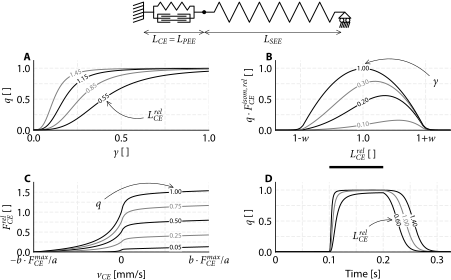
\includegraphics[keepaspectratio]{../figures/m_hill_model.pdf}}

}

\caption{\label{fig-m-hill-model}\textbf{Aspects of the Hill-type MTC
model used, illustrated at the top.} \(L_{CE}\), \(L_{PEE}\) and
\(L_{SEE}\) denote the CE, parallel elastic element (SEE) and serial
elastic element (SEE) length. CE represents the contractile part of the
muscle fibres, while PEE and SEE represent all elastic tissue in
parallel or in series, respectively, with CE. In the Hill-type MTC
model, CE force depends on active state (A), CE length (B) and CE
velocity (C). The effect of CE stimulation on active state (\(q\)) is
illustrated in D. A) The relationship between normalised free
\(Ca^{2+}\) concentration between the myofilaments (\(\gamma\)) and
\(q\). \(q\) also depends on relative CE length (\(L_{CE}^{rel}\)). B)
The product of \(q\) and the normalised active CE force-length
relationship for different values of \(\gamma\). C) The CE
force-velocity relationship for different values of \(q\). D) \(q\) over
time before, during and after CE stimulation for \(L_{CE}^{rel}=1\). CE
stimulation is maximal during the period indicated by the black bar and
`off' elsewhere.}

\end{figure}%

\subsection{\texorpdfstring{Simulated and \emph{in situ}
data}{Simulated and in situ data}}\label{simulated-and-in-situ-data}

\subsubsection{Simulated data}\label{sec-m-sim-data}

To simulate quick-release, step-ramp, and isometric experiments, we used
three parameter sets of a Hill-type MTC model from existing literature
for three rat m. gastrocnemius medialis (GM1, GM2, and GM3; see
\quartosupptblref{supptbl-overview}).

\textbf{Quick-release experiments} Each quick-release experiment
consisted of an isometric phase until SEE force plateaued, followed by a
rapid (step) change (10 ms) in MTC length and then followed by another
isometric phase (see Figure~\ref{fig-m-protocols}A). CE stimulation was
maximal (i.e., \(STIM = 1\)) during the first isometric phase and
continued at this maximal level until it was switched off shortly after
the step change in MTC length occurred. The step change in MTC length
was 0.2 mm and was chosen such that the resulting change in SEE force
was about 5-10\% of \(F_{CE}^{max}\). To prevent irreversible damage to
muscle fibres, the maximal MTC length used in experiments is typically
not far above the MTC length that yields maximal isometric SEE force
(\(L_{MTC}^{opt}\)). Accordingly, we simulated quick-release experiments
at various initial MTC lengths, ranging from a very short MTC length
(i.e., a length yielding very low isometric SEE force) and at every 1 mm
increment up to a MTC length that was maximal 3 mm above
\(L_{MTC}^{opt}\).

\textbf{Step-ramp experiments} Each step-ramp experiment consisted of an
isometric phase slightly above (\(\pm\) 0.5 mm) \(L_{MTC}^{opt}\),
followed by a rapid (step) change (10 ms) in MTC length and then a
constant MTC velocity ramp (see Figure~\ref{fig-m-protocols}B). CE
stimulation was maximal (i.e., \(STIM = 1\)) during the first isometric
phase and continued at this maximal level until it was switched off 0.1
s after the step change in MTC length occurred. The change in MTC length
of this step and the constant MTC velocity of the ramp were chosen such
that this resulted in a more or less a constant SEE force (and therefore
constant CE force) at the beginning of the ramp. We simulated 9
step-ramp experiments with different combinations of step sizes and
constant MTC velocity ramps, to cover a substantial part of the
concentric CE force-velocity relationship.

\textbf{Isometric experiments} Isometric experiments were simulated for
a combination of different MTC lengths (about 0, -2, -4 and -6 mm below
\(L_{MTC}^{opt}\)) and stimulation durations (35, 65 and 95 ms). CE
stimulation was maximal (i.e., \(STIM = 1\)) during the indicated
stimulation duration and fully off elsewhere (see
Figure~\ref{fig-m-protocols}C). The combination of four different MTC
lengths and three different stimulation durations resulted in twelve
different isometric experiments.

\begin{figure}[H]

\centering{

\pandocbounded{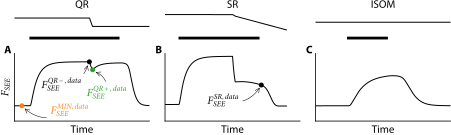
\includegraphics[keepaspectratio]{../figures/m_protocols.pdf}}

}

\caption{\label{fig-m-protocols}\textbf{Example of simulated data of
quick-release (A), step-ramp (B) and isometric (C) experiments.} Top:
MTC length over time. Bottom: SEE force over time. CE stimulation is
maximal during the period indicated by the black bar, and `off'
elsewhere. For each experiment, we obtained specific datapoints of SEE
force and the corresponding MTC length, which were used to estimate
contraction and excitation dynamics parameter values.}

\end{figure}%

\subsubsection{\texorpdfstring{\emph{In situ}
data}{In situ data}}\label{sec-m-insitu-data}

We also used data from an \emph{in situ} experiment on isolated rat m.
gastrocnemius medialis, conducted on three male Wistar rats. The
experiment included quick-release, step-ramp and isometric experiments,
which were similar to those described in Section~\ref{sec-m-sim-data}.
For each rat, we performed between 11 and 13 quick-release experiments,
10 and 12 step-ramp experiments and 12 isometric experiments. Below, we
provide a brief description of the experimental procedure, which is
fully detailed in (\citeproc{ref-reuvers_maximising_2025}{Reuvers et
al., 2025}).

In the experiment, approved by the Committee on the Ethics of Animal
Experimentation at the Vrije Universiteit (Permit Number: FBW-
AVD11200202114471), rats were first anesthetised with urethane. The
hindlimb was then shaved, and the overlying skin and m. biceps femoris
were removed. The medial and lateral part of m. gastrocnemius were
carefully separated from their surrounding tissue and exposed as much as
possible. The rats were placed in the experimental setup with the
hindlimb, femur and foot fully fixed. The distal end of the calcaneal
tendon was attached to a servomotor (Aurora 309C, Aurora Scientific,
Aurora, Canada) using Kevlar thread and aligned to ensure that m.
gastrocnemius medialis pulled in its natural direction. All nerves not
innervating m. gastrocnemius medialis were severed. M. gastrocnemius
medialis was stimulated via a cuff-electrode placed on the sciatic
nerve, with the proximal nerves crushed to prevent spinal reflexes. This
experimental setup allowed for precise control of m. gastrocnemius
medialis length changes and stimulation as well as accurate measurement
of m. gastrocnemius medialis force.

\subsection{Parameter value estimation
procedure}\label{sec-m-est-procedure}

The general procedure to estimate the parameter values involved
minimising the sum of squared differences between the data and the
values based on the estimated parameter values. To distinguish between
these, we used subscripts: for example, the value of the SEE force
before the quick-release of the data is indicated by
\(F_{SEE}^{QR-,data}\) while the value based on the estimated parameter
values is indicated by \(F_{SEE}^{QR-,est}\).

The data of the quick-release experiments were used to estimate the
parameter values of the CE, PEE and SEE force-length relationships. The
data of the step-ramp experiments were used to estimate the parameter
values of the CE force-velocity relationship. The data of the isometric
experiments were used to estimate the parameter values of the excitation
dynamics. Below we provide an overview on the methods used to estimate
the parameter values. We also offer an open-source toolbox that
automates the estimation of contraction and excitation dynamics
parameter values.

\subsubsection{CE, SEE and PEE force-length parameter value
estimation}\label{sec-m-estfl}

As explained in the introduction, different combinations of contraction
dynamics parameters can yield almost identical mechanical behaviour
under isometric conditions (see also Figure~\ref{fig-i-effect-ksee}).
For this reason, it is important to estimate SEE stiffness first, in
order to discriminate between SEE stiffness on the one hand, and
\(L_{CE}^{opt}\) and \(L_{SEE}^0\) on the other. In our approach, the
parameter that scales SEE stiffness (\(k_{SEE}\)) is therefore estimated
first. This is followed by the estimation of the PEE parameters, as
\(k_{SEE}\) is also required for their estimation. Finally, the
parameters \(F_{CE}^{max}\), \(L_{CE}^{opt}\), and \(L_{SEE}^0\) are
estimated.

\textbf{Estimation of SEE stiffness.} The first step was to estimate SEE
stiffness. The model SEE force depends on the parameter values of
\(k_{SEE}\) and \(L_{SEE}^0\), and obviously on SEE length. The problem,
however, is that SEE length is unknown in experiments. This makes it
challenging to estimate the parameter values concerning the SEE
force-length relationship. Fortunately, quick-release experiments
provide a way out. During quick-release experiments with a servomotor,
the motor quickly shortens MTC length such that there is a rapid decline
in SEE force (the `quick-release'). Due to the shortness of this
timeframe, CE shortening is minimal such that \emph{almost all} MTC
shortening is taken up by SEE. Often, in experimental studies, it is
assumed that \emph{all} MTC shortening can be attributed to SEE
shortening. In reality, this assumption leads to an overestimation of
SEE shortening, as CE also shortens during this short timeframe. We
introduced a method to correct for this overestimation of SEE shortening
(see Section~\ref{sec-m-im}) and estimated the parameter values
considering both methods: without and with correcting for CE shortening
during the quick-release.

Obtaining the SEE length change due to the quick-release
(\(\Delta L_{SEE}^{QR}\)) is a crucial step. This is because SEE length
after the quick-release (\(L_{SEE}^{QR+}\)) can then be expressed as SEE
length before the quick-release (\(L_{SEE}^{QR-}\)) plus the change in
SEE length due to the quick-release:
\(L_{SEE}^{QR+} = L_{SEE}^{QR-} + \Delta L_{SEE}^{QR}\). This allowed us
to rewrite Equation~\ref{eq-fee} to estimate SEE force immediately
before (\(F_{SEE}^{QR-,est}\)) and after (\(F_{SEE}^{QR+,est}\)) the
quick-release. This yielded:

\begin{equation}\phantomsection\label{eq-fseefit1}{
  \begin{split}
    F_{SEE}^{QR-,est}     &= k_{SEE} \cdot (L_{SEE}^{QR-} - L_{SEE}^0)^2 \\
    F_{SEE}^{QR+,est}     &= k_{SEE} \cdot (L_{SEE}^{QR-} + \Delta L_{SEE}^{QR} - L_{SEE}^0)^2
  \end{split}  
}\end{equation}

Now, there are two unknown parameters (i.e., \(k_{SEE}\) and
\(L_{SEE}^0\)), while also SEE length before the quick-release is also
unknown for each quick-release experiment. Consequently, there are more
unknowns than equations. To address this issue, we replaced
\(L_{SEE}^{QR-} - L_{SEE}^0\) with a temporary parameter \(c_{SEE}\).
This yielded:

\begin{equation}\phantomsection\label{eq-fseefit2}{
  \begin{split}
    F_{SEE}^{QR-,est}     &= k_{SEE} \cdot (c_{SEE})^2 \\
    F_{SEE}^{QR+,est}     &= k_{SEE} \cdot (c_{SEE} + \Delta L_{SEE}^{QR})^2
  \end{split}  
}\end{equation}

As \(k_{SEE}\) scales SEE stiffness, its value is constant across all
quick-release experiments. In contrast, \(c_{SEE}\) depends on the
parameter \(L_{SEE}^0\) and SEE length before the quick-release, which
differs among each quick-release experiment. Consequently, \(c_{SEE}\)
should be determined for each quick-release experiment individually.
Visually, \(c_{SEE}\) determines the shift along the x-axis on the SEE
force-length relationship, while \(k_{SEE}\) scales SEE stiffness and
consequently SEE force (see Figure~\ref{fig-m-ksee}A). The value of
\(k_{SEE}\) (and \(c_{SEE}\) for each quick-release experiment) were
found by minimising the sum of squared differences between the data and
estimated SEE force before (\(F_{SEE}^{QR-}\)) and after
(\(F_{SEE}^{QR+}\)) the quick-release.

\begin{figure}[H]

\centering{

\pandocbounded{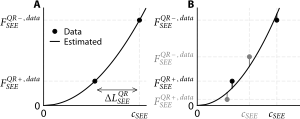
\includegraphics[keepaspectratio]{../figures/m_ksee.pdf}}

}

\caption{\label{fig-m-ksee}\textbf{Graphical illustration of SEE
stiffness parameter estimation.} For each quick-release experiment, SEE
force before (\(F_{SEE}^{QR-,data}\)) and after (\(F_{SEE}^{QR+,data}\))
the quick-release was obtained from the data, as well as the
corresponding decrease in SEE length (\(\Delta L_{SEE}^{QR}\)). Since
SEE length prior to the quick-release is typically unknown, a temporary
parameter (\(c_{SEE}\)) was introduced for each experiment to represent
the difference between SEE length before the quick-release and SEE slack
length. A) A single quick-release experiment yields two unknowns:
\(c_{SEE}\) and a parameter that scales SEE stiffness (\(k_{SEE}\)). B)
Running multiple quick-release experiments yields n+1 unknowns: n values
of \(c_{SEE}\) (one for each experiment) and the parameter scaling SEE
stiffness. Here, two quick-release experiments are illustrated (one
indicated with black dots, the other with grey dots), while the
estimated SEE force-length relationship is depicted with the black
line.}

\end{figure}%

\textbf{Estimation of PEE parameter values.} The second step was to
estimate PEE stiffness. The model PEE force depends on the parameter
values of \(k_{PEE}\) and \(L_{PEE}^0\), and obviously on PEE length. In
experiments, SEE force is measured, while PEE force is required to
estimate PEE stiffness. As such, experimental data should be used in
which CE force is negligible such that PEE force is approximately equal
to SEE force. At the beginning of the quick-release experiments, the
active state is so low that CE force is negligible. We selected an
interval of 10 ms in which the SEE force was minimal (\(F_{SEE}^{min}\),
orange dot in Figure~\ref{fig-m-protocols}A).

In experiments, PEE length is unknown. This problem can be addressed as
follows. First, PEE length equals MTC length minus SEE length:
\(L_{PEE} = L_{MTC} - L_{SEE}\) (Equation~\ref{eq-lcelseelmtc}). Second,
SEE length is the sum of SEE slack length and SEE elongation
(\(E_{SEE}\): \(L_{SEE} = L_{SEE}^0 + E_{SEE}\)). This allowed us to
rewrite Equation~\ref{eq-fee} to estimate PEE force (\(F_{PEE}^{est}\)),
yielding:

\begin{equation}\phantomsection\label{eq-fpeefit1}{
F_{PEE}^{est} = k_{PEE} \cdot (L_{MTC} -  - L_{SEE}^0 - E_{SEE} - L_{PEE}^0)^2
}\end{equation}

Now, there are two unknown parameter values (i.e., \(k_{PEE}\) and
\(L_{PEE}^0\)), while also SEE elongation is unknown for every
quick-release experiment. Consequently, there are more unknowns than
equations. To address this, we replaced \(L_{PEE}^0 + L_{SEE}^0\) with a
temporary parameter \(c_{PEE}\). Subsequently, SEE elongation was
computed as \(\sqrt{\frac{F_{SEE}^{MIN,data}}{k_{SEE}}}\), given the
estimated SEE stiffness scaling factor in the previous step. This
yielded:

\begin{equation}\phantomsection\label{eq-fpeefit2}{
F_{PEE}^{est} = k_{PEE} \cdot (L_{MTC} - \sqrt{\frac{F_{SEE}^{MIN,data}}{k_{SEE}}} - c_{PEE})^2
}\end{equation}

As \(k_{PEE}\) only scales PEE stiffness, its value is constant across
all quick-release experiments. Similarly, \(c_{PEE}\) is the sum of
\(L_{SEE}^0\) and \(L_{PEE}^0\) and should therefore be constant for
each quick-release experiment. The values of \(k_{PEE}\) and \(c_{PEE}\)
were then computed by minimising the sum of squared differences between
\(F_{PEE}^{est}\) and \(F_{SEE}^{min,data}\).

\textbf{Estimation of \(F_{CE}^{max}\), \(L_{CE}^{opt}\) and
\(L_{SEE}^0\).} The third step was to estimate \(F_{CE}^{max}\),
\(L_{CE}^{opt}\) and \(L_{SEE}^0\). Before the quick-release, MTC is
isometrically delivering force. We used the SEE force at this instant
(\(F_{SEE}^{QR-,data}\), black dot in Figure~\ref{fig-m-protocols}A) and
the corresponding MTC length to obtain the MTC force-length relationship
from the data. We then estimated maximal isometric CE force
(\(F_{CE}^{max}\)), CE optimum length (\(L_{CE}^{opt}\)) and SEE slack
length (\(L_{SEE}^0\)) by minimising the sum of squared differences
between the data and estimated MTC force-length relationship. Lastly,
\(L_{PEE}^0\) was computed by subtracting \(L_{SEE}^0\) from
\(c_{PEE}\).

\subsubsection{CE force-velocity parameter value
estimation}\label{sec-m-estfv}

The values of the CE force--velocity relationship parameters \(a\) and
\(b\) were estimated from data obtained during the plateau phase of SEE
force in step-ramp experiments. This approach was chosen because SEE
length is constant when SEE force is constant. Consequently, CE velocity
equals MTC velocity under these conditions. Following this argument, we
first identified a 10\,ms interval in which SEE force changed the least.
Second, we derived CE length and CE force as functions of time using
Equation~\ref{eq-lcelseelmtc} and Equation~\ref{eq-fee}. Third, we
calculated the CE velocity as the time-derivative of CE length. Finally,
we averaged CE force and CE velocity over the 10\,ms interval. This
procedure yielded the data of the CE force-velocity relationship.

Now, the model CE force-velocity relationship can be fit to that of the
data to obtain value of \(a\) and \(b\). However, employing a method
that simply minimises the sum of ordinary least squares differences
would not be appropriate because in experiments there is uncertainty in
both measured CE force and CE velocity. Instead, we used a total least
squares method that minimised the distance between the modelled CE force
(\(F_{CE}^{est}\)) and CE velocity (\(v_{CE}^{est}\)) (now called: model
values) and those of the data (see also Figure~\ref{fig-m-fv}). To do
this, we had to find the nearest model values to the CE force of the
data (\(F_{CE}^{data}\)) and CE velocity of the data (\(v_{CE}^{data}\))
(now called: datapoints). We used the following observations: 1) the
model value has to satisfy Equation~\ref{eq-fvcon} and 2) the derivative
of \(\frac{dF_{CE}}{dv_{CE}}\) of the model value should be
perpendicular to the line from the datapoint to the model value (see
Figure~\ref{fig-m-fv}). Hence, the model value could be found by solving
Equation~\ref{eq-fvcon} and Equation~\ref{eq-fvperpline}:

\begin{equation}\phantomsection\label{eq-fvperpline}{
  \frac{dv_{CE}^{est}}{dF_{CE}^{est}} \cdot (v_{CE}^{est} - v_{CE}^{data}) = F_{CE}^{data} - F_{CE}^{est}
}\end{equation}

The following cost-function was then minimised to find the parameter
values of \(a\) and \(b\):

\[
  J = \sum_{i=1}^{n} {\biggl(\frac{F_{CE}^{data} - F_{CE}^{est}}{c_1}\biggr)}^2 + {\biggl(\frac{v_{CE}^{data} - v_{CE}^{est}}{c_2}\biggr)}^2
\]

\(c_1\) and \(c_2\) denote scaling factors such that both terms of the
cost-function are more or less equally weighted, which was done by
setting \(c_1\) equal to the maximal range in CE force of the data and
setting \(c_2\) equal to the maximal range of CE velocity of the data.

\begin{figure}[H]

\centering{

\pandocbounded{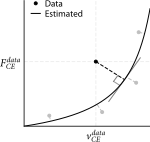
\includegraphics[keepaspectratio]{../figures/m_fv.pdf}}

}

\caption{\label{fig-m-fv}\textbf{Graphical illustration of the CE
force-velocity parameter estimation using total least squares.} For each
step-ramp experiment, CE force and CE velocity was obtained during the
interval in which SEE force changed the least. The nearest point on the
CE force-velocity relationship was identified based on two criteria: it
should satisfy Equation~\ref{eq-fvcon}, and the line from the datapoint
to the CE force-velocity relationship should be perpendicular the CE
force-velocity relationship. This was done for all step-ramp experiments
(other datapoints are depicted in grey), while the estimated CE
force-velocity relationshp is depicted with the black line.}

\end{figure}%

\subsubsection{Excitation dynamics parameter value
estimation}\label{excitation-dynamics-parameter-value-estimation}

We estimated the parameters values of \(\tau_{act}\) and
\(\tau_{deact}\) based on isometric experiments. The choice to estimate
only these parameters of the excitation dynamics was made because it is
generally challenging to discriminate between parameter values of both
the calcium dynamics (Equation~\ref{eq-gammad}) and the \(q-[Ca^{2+}]\)
relation (Equation~\ref{eq-activestate}) based on mechanical
measurements outlined above. The parameter values of the \(q-[Ca^{2+}]\)
relation were set to those used in simulating the isometric experiments.
Consequently, these parameters matched their actual values for the
simulated data, but obviously were suboptimal for the \emph{in situ}
data. To estimate the parameter values of \(\tau_{act}\) and
\(\tau_{deact}\), we minimised the sum of squared differences between
the SEE force of the data and the estimated SEE force based on the
parameter values. For this, an interval of the data was used starting
from maximal CE stimulation to 0.1 s after CE stimulation ceased off.

\subsubsection{Parameter estimation: traditional method \& improved
method}\label{sec-m-im}

To estimate the SEE stiffness it is generally assumed that the
quick-release is so fast that all MTC shortening is taken up by SEE. As
A.V. Hill already acknowledged in
(\citeproc{ref-hill_series_1950}{1950}), this is not the case in reality
as CE also shortens. Although this CE shortening might be small, SEE is
in general stiff and therefore small errors in SEE length may result in
large errors in predicted SEE forces and thus in estimated SEE
stiffness. We used two different methods to estimate the parameter
values: 1) the traditional method and the improved method. In the
traditional method, we followed the procedure outlined in section
Section~\ref{sec-m-estfl} and Section~\ref{sec-m-estfv}. In the improved
method, we also followed the procedure outlined in
Section~\ref{sec-m-estfl} and Section~\ref{sec-m-estfv} after which we
incorporated an additional procedure to correct for CE shortening due to
the quick-release. This additional procedure was as follows: 1) We
calculated CE length just before the (step) change in MTC length
occurred using Equation~\ref{eq-lcelseelmtc}, \ref{eq-fee},
\ref{eq-forcelength} and \ref{eq-activestate}, assuming that CE velocity
was 0 and that \(\gamma\) equalled 1. 2) We performed a (short)
simulation from the time just before the (step) change in MTC length to
just after the (step) change in MTC length. 3) We computed the change in
CE length over this time interval as the average CE length slightly
before and slightly after the (step) change in MTC length. 4) We
subtracted the change in CE length from the change in MTC length to
obtain the change in SEE length. In addition to correcting for CE length
change during the quick-release, we incorporated a step to obtain better
estimates of the actual PEE force at the time instance of minimum SEE
force (\(F_{SEE}^{min,data}\); see Figure~\ref{fig-m-protocols}). We
computed CE force at this time instance using
Equation~\ref{eq-forcelength} and \ref{eq-activestate}, assuming that
\(\gamma\) equalled its minimum value. This CE force was then subtracted
from \(F_{SEE}^{min,data}\).

The improved method leads to a different (i.e., higher) SEE stiffness,
which affect the estimation of the parameter values of the CE, PEE and
SEE force-length relationships (see Section~\ref{sec-m-estfl}). These
estimated parameter values were then used to again estimate the
parameter values of the CE force-velocity relationship (see section
Section~\ref{sec-m-estfv}). As the parameter values of the CE
force-velocity relationship slightly changed, the estimate of CE length
change due to the quick-release also changed and therefore estimated SEE
stiffness changed. We found that this process always converged to a
stable solution and therefore we used an iterative process until the
change in all parameter values was less than 0.1\% (see
\quartosuppfigref{suppfig-flowchart}).

\subsection{Sensitivity analysis}\label{sec-m-sa}

\subsubsection{Monte Carlo simulations}\label{monte-carlo-simulations}

In experiments on isolated MTC, the MTC force-length relationship can
shift due to irreversible damage of SEE
(\citeproc{ref-aubert_tension-length_1951}{Aubert et al., 1951}). We
observed this phenomenon in an experiment involving isolated rat m.
gastrocnemius medialis, where the MTC force-length relationship shifted
by about 1 mm (\textasciitilde8\% \(L_{CE}^{opt}\)) over a period of
approximately 8 hours (Reuvers et al., unpublished observation). To
assess the influence of these shifts on the parameter value estimation,
we performed Monte Carlo simulations. We assumed that the observed
shifts of the MTC force-length relationship were caused solely by a
decrease in SEE stiffness. Accordingly, we decreased SEE stiffness to
cause random shifts of the MTC force-length relationship between 0 and 1
mm. This way, we simulated data as if they were collected at random
intervals throughout an 8-hour period. Importantly, changes in SEE
stiffness affect the step size and constant MTC velocity ramp required
for a more or less a constant SEE force at the beginning of the ramp in
step-ramp experiments. Therefore, we adjusted the step size and constant
MTC velocity ramp for each simulated step-ramp trial individually.
Parameter values of each MTC were then estimated using the `perturbed'
data using the improved method (see Section~\ref{sec-m-im}). This
process was repeated 50 times for each MTC, allowing us to evaluate both
the mean and the spread of the estimated parameter values.

\subsubsection{Interdependency of parameter
values}\label{interdependency-of-parameter-values}

The parameter estimation procedure detailed above follows a fixed order
in which certain parameters are estimated before others. For instance,
\(k_{SEE}\) is estimated first and therefore affects the estimation of
\(L_{SEE}^0\) and \(L_{CE}^{opt}\). This sequence creates an
interdependency among the parameter values, which has been identified as
a potential cause for substantial variation in parameter values among
individuals, even within the same muscle type
(\citeproc{ref-lemaire_comparison_2016}{Lemaire et al., 2016}). To
investigate this interdependency, we systematically changed parameter
values of our model. Specifically, we increased and decreased each
parameter value by 5\% relative to the values obtained with the improved
method. After this, we re-estimated all other parameter values. This
approach allowed us to assess the influence of changes in one parameter
on the estimation of others.

\section{Results}\label{results}

\subsection{Evaluating parameter value estimation accuracy - simulated
data}\label{evaluating-parameter-value-estimation-accuracy---simulated-data}

\begin{Shaded}
\begin{Highlighting}[]
\CommentTok{\# \%\% Load packages}
\ImportTok{import}\NormalTok{ os, pickle, sys}
\ImportTok{import}\NormalTok{ numpy }\ImportTok{as}\NormalTok{ np}
\ImportTok{import}\NormalTok{ pandas }\ImportTok{as}\NormalTok{ pd}
\ImportTok{from}\NormalTok{ pathlib }\ImportTok{import}\NormalTok{ Path}

\CommentTok{\# Set directories}
\NormalTok{cwd }\OperatorTok{=}\NormalTok{ Path.cwd()}
\NormalTok{baseDir }\OperatorTok{=}\NormalTok{ cwd.parent}
\NormalTok{dataDir }\OperatorTok{=}\NormalTok{ baseDir }\OperatorTok{/} \StringTok{\textquotesingle{}data\textquotesingle{}}
\NormalTok{funcDir }\OperatorTok{=}\NormalTok{ baseDir }\OperatorTok{/} \StringTok{\textquotesingle{}analysis\textquotesingle{}} \OperatorTok{/} \StringTok{\textquotesingle{}functions\textquotesingle{}}
\NormalTok{sys.path.append(}\BuiltInTok{str}\NormalTok{(funcDir))}

\CommentTok{\# Custom functions}
\ImportTok{import}\NormalTok{ hillmodel, stats}

\CommentTok{\# \%\% Extract parameters}
\NormalTok{muscles }\OperatorTok{=}\NormalTok{ [}\StringTok{\textquotesingle{}GMs1\textquotesingle{}}\NormalTok{,}\StringTok{\textquotesingle{}GMs2\textquotesingle{}}\NormalTok{,}\StringTok{\textquotesingle{}GMs3\textquotesingle{}}\NormalTok{]}
\NormalTok{param\_keys }\OperatorTok{=}\NormalTok{ [}\StringTok{\textquotesingle{}a\textquotesingle{}}\NormalTok{, }\StringTok{\textquotesingle{}b\textquotesingle{}}\NormalTok{, }\StringTok{\textquotesingle{}kpee\textquotesingle{}}\NormalTok{, }\StringTok{\textquotesingle{}ksee\textquotesingle{}}\NormalTok{, }\StringTok{\textquotesingle{}fmax\textquotesingle{}}\NormalTok{, }\StringTok{\textquotesingle{}lce\_opt\textquotesingle{}}\NormalTok{, }\StringTok{\textquotesingle{}lpee0\textquotesingle{}}\NormalTok{, }\StringTok{\textquotesingle{}lsee0\textquotesingle{}}\NormalTok{, }\StringTok{\textquotesingle{}tact\textquotesingle{}}\NormalTok{, }\StringTok{\textquotesingle{}tdeact\textquotesingle{}}\NormalTok{]}

\NormalTok{orParms, tmParms, imParms }\OperatorTok{=}\NormalTok{ [], [], []}
\ControlFlowTok{for}\NormalTok{ mus }\KeywordTok{in}\NormalTok{ muscles:   }
\NormalTok{    orPar }\OperatorTok{=}\NormalTok{ pickle.load(}\BuiltInTok{open}\NormalTok{(os.path.join(dataDir,mus,}\StringTok{\textquotesingle{}parameters\textquotesingle{}}\NormalTok{,mus}\OperatorTok{+}\StringTok{\textquotesingle{}\_OR.pkl\textquotesingle{}}\NormalTok{), }\StringTok{\textquotesingle{}rb\textquotesingle{}}\NormalTok{))}
\NormalTok{    tmPar }\OperatorTok{=}\NormalTok{ pickle.load(}\BuiltInTok{open}\NormalTok{(os.path.join(dataDir,mus,}\StringTok{\textquotesingle{}parameters\textquotesingle{}}\NormalTok{,mus}\OperatorTok{+}\StringTok{\textquotesingle{}\_TM.pkl\textquotesingle{}}\NormalTok{), }\StringTok{\textquotesingle{}rb\textquotesingle{}}\NormalTok{))[}\DecValTok{0}\NormalTok{]}
\NormalTok{    imPar }\OperatorTok{=}\NormalTok{ pickle.load(}\BuiltInTok{open}\NormalTok{(os.path.join(dataDir,mus,}\StringTok{\textquotesingle{}parameters\textquotesingle{}}\NormalTok{,mus}\OperatorTok{+}\StringTok{\textquotesingle{}\_IM.pkl\textquotesingle{}}\NormalTok{), }\StringTok{\textquotesingle{}rb\textquotesingle{}}\NormalTok{))[}\DecValTok{0}\NormalTok{]}

\NormalTok{    parms }\OperatorTok{=}\NormalTok{ [orPar[k] }\ControlFlowTok{for}\NormalTok{ k }\KeywordTok{in}\NormalTok{ param\_keys]}
\NormalTok{    orParms.append(parms)}
    
\NormalTok{    parms }\OperatorTok{=}\NormalTok{ [tmPar[k] }\ControlFlowTok{for}\NormalTok{ k }\KeywordTok{in}\NormalTok{ param\_keys]}
\NormalTok{    tmParms.append(parms)}
    
\NormalTok{    parms }\OperatorTok{=}\NormalTok{ [imPar[k] }\ControlFlowTok{for}\NormalTok{ k }\KeywordTok{in}\NormalTok{ param\_keys]}
\NormalTok{    imParms.append(parms)}
    
\CommentTok{\# Store in pandas dataframe}
\NormalTok{df\_or }\OperatorTok{=}\NormalTok{ pd.DataFrame(}\BuiltInTok{list}\NormalTok{(}\BuiltInTok{zip}\NormalTok{(}\OperatorTok{*}\NormalTok{orParms)), columns}\OperatorTok{=}\NormalTok{[}\StringTok{\textquotesingle{}GM1\textquotesingle{}}\NormalTok{, }\StringTok{\textquotesingle{}GM2\textquotesingle{}}\NormalTok{, }\StringTok{\textquotesingle{}GM3\textquotesingle{}}\NormalTok{], index}\OperatorTok{=}\NormalTok{param\_keys) }\CommentTok{\# df with actual/real parameter values}
\NormalTok{df\_tm }\OperatorTok{=}\NormalTok{ pd.DataFrame(}\BuiltInTok{list}\NormalTok{(}\BuiltInTok{zip}\NormalTok{(}\OperatorTok{*}\NormalTok{tmParms)), columns}\OperatorTok{=}\NormalTok{[}\StringTok{\textquotesingle{}GM1\textquotesingle{}}\NormalTok{, }\StringTok{\textquotesingle{}GM2\textquotesingle{}}\NormalTok{, }\StringTok{\textquotesingle{}GM3\textquotesingle{}}\NormalTok{], index}\OperatorTok{=}\NormalTok{param\_keys) }\CommentTok{\# df with estimated parameter values using the traditional method}
\NormalTok{df\_im }\OperatorTok{=}\NormalTok{ pd.DataFrame(}\BuiltInTok{list}\NormalTok{(}\BuiltInTok{zip}\NormalTok{(}\OperatorTok{*}\NormalTok{imParms)), columns}\OperatorTok{=}\NormalTok{[}\StringTok{\textquotesingle{}GM1\textquotesingle{}}\NormalTok{, }\StringTok{\textquotesingle{}GM2\textquotesingle{}}\NormalTok{, }\StringTok{\textquotesingle{}GM3\textquotesingle{}}\NormalTok{], index}\OperatorTok{=}\NormalTok{param\_keys) }\CommentTok{\# df with estimated parameter values using the improved method}

\CommentTok{\# \%\% Compute percentage differences from real/actual and estimated parameter values}
\CommentTok{\# Positive: Estimated is that \% higher than Real}
\CommentTok{\# Negative: Estimated is that \% lower than Real}
\NormalTok{df\_tm\_p }\OperatorTok{=}\NormalTok{ stats.pdiff(df\_tm, df\_or)}
\NormalTok{df\_im\_p }\OperatorTok{=}\NormalTok{ stats.pdiff(df\_im, df\_or)}

\CommentTok{\# \%\% Variables related to overestimation of length changes due to QR}
\NormalTok{deltaLsee\_tm   }\OperatorTok{=}\NormalTok{ np.full((}\BuiltInTok{len}\NormalTok{(muscles),}\DecValTok{10}\NormalTok{), np.nan)}
\NormalTok{deltaLsee\_real }\OperatorTok{=}\NormalTok{ np.full((}\BuiltInTok{len}\NormalTok{(muscles),}\DecValTok{10}\NormalTok{), np.nan)}
\ControlFlowTok{for}\NormalTok{ iMus,mus }\KeywordTok{in} \BuiltInTok{enumerate}\NormalTok{(muscles):   }
\NormalTok{    orPar }\OperatorTok{=}\NormalTok{ pickle.load(}\BuiltInTok{open}\NormalTok{(os.path.join(dataDir,mus,}\StringTok{\textquotesingle{}parameters\textquotesingle{}}\NormalTok{,mus}\OperatorTok{+}\StringTok{\textquotesingle{}\_OR.pkl\textquotesingle{}}\NormalTok{), }\StringTok{\textquotesingle{}rb\textquotesingle{}}\NormalTok{))}
\NormalTok{    tmPar,dataQRtm }\OperatorTok{=}\NormalTok{ pickle.load(}\BuiltInTok{open}\NormalTok{(os.path.join(dataDir,mus,}\StringTok{\textquotesingle{}parameters\textquotesingle{}}\NormalTok{,mus}\OperatorTok{+}\StringTok{\textquotesingle{}\_TM.pkl\textquotesingle{}}\NormalTok{), }\StringTok{\textquotesingle{}rb\textquotesingle{}}\NormalTok{))[}\DecValTok{0}\NormalTok{:}\DecValTok{2}\NormalTok{]}

\NormalTok{    fseeQRpre }\OperatorTok{=}\NormalTok{ dataQRtm[}\StringTok{\textquotesingle{}fseeQRpre\textquotesingle{}}\NormalTok{]}
\NormalTok{    fseeQRpst }\OperatorTok{=}\NormalTok{ dataQRtm[}\StringTok{\textquotesingle{}fseeQRpst\textquotesingle{}}\NormalTok{]}
\NormalTok{    lseeQRpre }\OperatorTok{=}\NormalTok{ (fseeQRpre}\OperatorTok{/}\NormalTok{orPar[}\StringTok{\textquotesingle{}ksee\textquotesingle{}}\NormalTok{])}\OperatorTok{**}\FloatTok{0.5} \OperatorTok{+}\NormalTok{ orPar[}\StringTok{\textquotesingle{}lsee0\textquotesingle{}}\NormalTok{]}
\NormalTok{    lseeQRpst }\OperatorTok{=}\NormalTok{ (fseeQRpst}\OperatorTok{/}\NormalTok{orPar[}\StringTok{\textquotesingle{}ksee\textquotesingle{}}\NormalTok{])}\OperatorTok{**}\FloatTok{0.5} \OperatorTok{+}\NormalTok{ orPar[}\StringTok{\textquotesingle{}lsee0\textquotesingle{}}\NormalTok{]}
    
    \CommentTok{\# Compute change in SEE length due to QR}
\NormalTok{    deltaLsee\_tm[iMus] }\OperatorTok{=}\NormalTok{ dataQRtm[}\StringTok{\textquotesingle{}lseeQRpre\textquotesingle{}}\NormalTok{]}\OperatorTok{{-}}\NormalTok{dataQRtm[}\StringTok{\textquotesingle{}lseeQRpst\textquotesingle{}}\NormalTok{]  }\CommentTok{\# [m] estimated SEE length change due to QR}
\NormalTok{    deltaLsee\_real[iMus] }\OperatorTok{=}\NormalTok{ lseeQRpre}\OperatorTok{{-}}\NormalTok{lseeQRpst  }\CommentTok{\# [m] real/actual SEE length change due to QR}

\CommentTok{\# Compute percentage difference from real to estimated SEE length change due to QR}
\CommentTok{\# Positive: TM is that \% higher than Real}
\CommentTok{\# Negative: TM is that \% lower than Real}
\NormalTok{p\_deltaLsee }\OperatorTok{=}\NormalTok{ stats.pdiff(deltaLsee\_tm, deltaLsee\_real)  }\CommentTok{\# [\%] percentage difference }
\NormalTok{p\_deltaLseeAvg }\OperatorTok{=}\NormalTok{ np.mean(p\_deltaLsee,}\DecValTok{1}\NormalTok{)  }\CommentTok{\# [\%] average per muscle}
\NormalTok{p\_deltaLseeStd }\OperatorTok{=}\NormalTok{ np.std(p\_deltaLsee,}\DecValTok{1}\NormalTok{)  }\CommentTok{\# [\%] std per muscle}

\CommentTok{\# Compute difference between real and estimated CE length change due to QR}
\NormalTok{deltaLce }\OperatorTok{=}\NormalTok{ deltaLsee\_real}\OperatorTok{{-}}\NormalTok{deltaLsee\_tm  }\CommentTok{\# [m]}
\NormalTok{deltaLceAvg }\OperatorTok{=}\NormalTok{ np.mean(deltaLce,}\DecValTok{1}\NormalTok{)  }\CommentTok{\# [m] average per muscle}
\NormalTok{deltaLceStd }\OperatorTok{=}\NormalTok{ np.std(deltaLce,}\DecValTok{1}\NormalTok{)  }\CommentTok{\# [m] std per muscle}

\CommentTok{\# \%\% 3.1.1: Traditional vs. Improved method}
\CommentTok{\# Extract all contraction dynamics parameters except ksee}
\NormalTok{p\_TM\_con }\OperatorTok{=}\NormalTok{ df\_tm\_p.loc[[}\StringTok{\textquotesingle{}a\textquotesingle{}}\NormalTok{,}\StringTok{\textquotesingle{}b\textquotesingle{}}\NormalTok{, }\StringTok{\textquotesingle{}kpee\textquotesingle{}}\NormalTok{, }\StringTok{\textquotesingle{}fmax\textquotesingle{}}\NormalTok{, }\StringTok{\textquotesingle{}lce\_opt\textquotesingle{}}\NormalTok{, }\StringTok{\textquotesingle{}lpee0\textquotesingle{}}\NormalTok{, }\StringTok{\textquotesingle{}lsee0\textquotesingle{}}\NormalTok{]]}

\CommentTok{\# Avg. difference: from real to estimated SEE length change}
\NormalTok{p\_TM\_deltaLsee\_avgall }\OperatorTok{=} \SpecialStringTok{f\textquotesingle{}}\SpecialCharTok{\{}\NormalTok{p\_deltaLseeAvg}\SpecialCharTok{.}\NormalTok{mean()}\SpecialCharTok{:0.0f\}}\SpecialStringTok{\textquotesingle{}} \CommentTok{\#  [\%] avg. percentage difference}
\CommentTok{\# Avg. difference over all muscles: from real to estimated SEE stiffness}
\NormalTok{p\_TM\_ksee\_avg }\OperatorTok{=} \SpecialStringTok{f\textquotesingle{}}\SpecialCharTok{\{}\NormalTok{df\_tm\_p}\SpecialCharTok{.}\NormalTok{loc[}\StringTok{\textquotesingle{}ksee\textquotesingle{}}\NormalTok{]}\SpecialCharTok{.}\NormalTok{mean()}\SpecialCharTok{:0.0f\}}\SpecialStringTok{\textquotesingle{}} \CommentTok{\#  [\%] avg. percentage difference}
\CommentTok{\# Avg. difference over all muscles: from real to estimated tact}
\NormalTok{p\_TM\_tact\_avg }\OperatorTok{=} \SpecialStringTok{f\textquotesingle{}}\SpecialCharTok{\{}\NormalTok{df\_tm\_p}\SpecialCharTok{.}\NormalTok{loc[}\StringTok{\textquotesingle{}tact\textquotesingle{}}\NormalTok{]}\SpecialCharTok{.}\NormalTok{mean()}\SpecialCharTok{:0.0f\}}\SpecialStringTok{\%\textquotesingle{}}  \CommentTok{\# [\%] avg. percentage difference}
\CommentTok{\# Max. difference over all muscles: from real to estimated tact}
\NormalTok{p\_TM\_con\_max }\OperatorTok{=} \SpecialStringTok{f\textquotesingle{}}\SpecialCharTok{\{}\NormalTok{p\_TM\_con}\SpecialCharTok{.}\BuiltInTok{abs}\NormalTok{()}\SpecialCharTok{.}\BuiltInTok{max}\NormalTok{()}\SpecialCharTok{.}\BuiltInTok{max}\NormalTok{()}\SpecialCharTok{:0.1f\}}\SpecialStringTok{\textquotesingle{}}  \CommentTok{\# [\%] max. percentage difference}
\CommentTok{\# Max. difference over all muscles: from real to estimated tact}
\NormalTok{p\_IM\_max }\OperatorTok{=} \SpecialStringTok{f\textquotesingle{}}\SpecialCharTok{\{}\NormalTok{df\_im\_p}\SpecialCharTok{.}\BuiltInTok{abs}\NormalTok{()}\SpecialCharTok{.}\BuiltInTok{max}\NormalTok{()}\SpecialCharTok{.}\BuiltInTok{max}\NormalTok{()}\SpecialCharTok{:0.0f\}}\SpecialStringTok{\textquotesingle{}}  \CommentTok{\# [\%] max. percentage difference}

\CommentTok{\# \%\% 3.1.2: Estimation of SEE stiffness. }
\CommentTok{\# Difference between SEE elongation of estimated parameter value and real/actual value}
\CommentTok{\# Positive: estimated value is higher than real/actual value}
\NormalTok{d\_esee }\OperatorTok{=}\NormalTok{ (df\_tm.loc[}\StringTok{\textquotesingle{}fmax\textquotesingle{}}\NormalTok{]}\OperatorTok{/}\NormalTok{df\_tm.loc[}\StringTok{\textquotesingle{}ksee\textquotesingle{}}\NormalTok{])}\OperatorTok{**}\FloatTok{0.5} \OperatorTok{{-}}\NormalTok{ (df\_or.loc[}\StringTok{\textquotesingle{}fmax\textquotesingle{}}\NormalTok{]}\OperatorTok{/}\NormalTok{df\_or.loc[}\StringTok{\textquotesingle{}ksee\textquotesingle{}}\NormalTok{])}\OperatorTok{**}\FloatTok{0.5} \CommentTok{\# [m]}

\CommentTok{\# Correlation coefficients}
\NormalTok{r\_see }\OperatorTok{=}\NormalTok{ np.full(}\BuiltInTok{len}\NormalTok{(muscles), np.nan)}
\NormalTok{r\_pee }\OperatorTok{=}\NormalTok{ np.full(}\BuiltInTok{len}\NormalTok{(muscles), np.nan)}
\NormalTok{r\_mtc }\OperatorTok{=}\NormalTok{ np.full(}\BuiltInTok{len}\NormalTok{(muscles), np.nan)}
\ControlFlowTok{for}\NormalTok{ iMus,mus }\KeywordTok{in} \BuiltInTok{enumerate}\NormalTok{(muscles):   }
\NormalTok{    parFile }\OperatorTok{=}\NormalTok{ os.path.join(dataDir,mus,}\StringTok{\textquotesingle{}parameters\textquotesingle{}}\NormalTok{,mus}\OperatorTok{+}\StringTok{\textquotesingle{}\_TM.pkl\textquotesingle{}}\NormalTok{)}
\NormalTok{    muspar, dataQR, dataSR, dataACTout }\OperatorTok{=}\NormalTok{ pickle.load(}\BuiltInTok{open}\NormalTok{(parFile, }\StringTok{\textquotesingle{}rb\textquotesingle{}}\NormalTok{))}
    
    \CommentTok{\# SEE}
\NormalTok{    lseeData }\OperatorTok{=}\NormalTok{ np.hstack((dataQR[}\StringTok{\textquotesingle{}lseeQRpre\textquotesingle{}}\NormalTok{],dataQR[}\StringTok{\textquotesingle{}lseeQRpst\textquotesingle{}}\NormalTok{]))}
\NormalTok{    fseeData }\OperatorTok{=}\NormalTok{ np.hstack((dataQR[}\StringTok{\textquotesingle{}fseeQRpre\textquotesingle{}}\NormalTok{],dataQR[}\StringTok{\textquotesingle{}fseeQRpst\textquotesingle{}}\NormalTok{]))}
\NormalTok{    fseeMdl }\OperatorTok{=}\NormalTok{ hillmodel.LEE2Force(lseeData,}\DecValTok{0}\NormalTok{,muspar)[}\DecValTok{0}\NormalTok{]}
\NormalTok{    r\_see[iMus] }\OperatorTok{=}\NormalTok{ np.corrcoef(fseeData, fseeMdl)[}\DecValTok{0}\NormalTok{,}\DecValTok{1}\NormalTok{]}
    
    \CommentTok{\# PEE}
\NormalTok{    fpeeMdl }\OperatorTok{=}\NormalTok{ hillmodel.LEE2Force(}\DecValTok{0}\NormalTok{,dataQR[}\StringTok{\textquotesingle{}lpeeQR\textquotesingle{}}\NormalTok{],muspar)[}\DecValTok{1}\NormalTok{]}
\NormalTok{    r\_pee[iMus] }\OperatorTok{=}\NormalTok{ np.corrcoef(dataQR[}\StringTok{\textquotesingle{}fpeeQR\textquotesingle{}}\NormalTok{], fpeeMdl)[}\DecValTok{0}\NormalTok{,}\DecValTok{1}\NormalTok{]}
    
    \CommentTok{\# MTC}
\NormalTok{    fseeMdl }\OperatorTok{=}\NormalTok{ hillmodel.ForceEQ(dataQR[}\StringTok{\textquotesingle{}lmtcQRpre\textquotesingle{}}\NormalTok{],}\DecValTok{1}\NormalTok{,muspar)[}\DecValTok{0}\NormalTok{]}
\NormalTok{    r\_mtc[iMus] }\OperatorTok{=}\NormalTok{ np.corrcoef(dataQR[}\StringTok{\textquotesingle{}fseeQRpre\textquotesingle{}}\NormalTok{], fseeMdl)[}\DecValTok{0}\NormalTok{,}\DecValTok{1}\NormalTok{]}
\NormalTok{r\_all }\OperatorTok{=}\NormalTok{ np.hstack((r\_see,r\_pee,r\_mtc))}

\CommentTok{\# Percentage difference from real to estimated parameter}
\NormalTok{p\_TM\_ksee }\OperatorTok{=}\NormalTok{ [}\SpecialStringTok{f\textquotesingle{}}\SpecialCharTok{\{}\NormalTok{v}\SpecialCharTok{:0.0f\}}\SpecialStringTok{\textquotesingle{}} \ControlFlowTok{for}\NormalTok{ v }\KeywordTok{in}\NormalTok{ df\_tm\_p.loc[}\StringTok{\textquotesingle{}ksee\textquotesingle{}}\NormalTok{]]  }\CommentTok{\# [\%] per muscle}
\CommentTok{\# Avg\&Std per muscle: differences from real to estimated parameters }
\NormalTok{p\_TM\_deltaLsee\_avgmus }\OperatorTok{=}\NormalTok{ [}\SpecialStringTok{f\textquotesingle{}}\SpecialCharTok{\{}\NormalTok{v}\SpecialCharTok{:0.0f\}}\SpecialStringTok{\textquotesingle{}} \ControlFlowTok{for}\NormalTok{ v }\KeywordTok{in}\NormalTok{ p\_deltaLseeAvg]  }\CommentTok{\# [\%]}
\NormalTok{p\_TM\_deltaLsee\_stdmus }\OperatorTok{=}\NormalTok{ [}\SpecialStringTok{f\textquotesingle{}}\SpecialCharTok{\{}\NormalTok{v}\SpecialCharTok{:0.0f\}}\SpecialStringTok{\textquotesingle{}} \ControlFlowTok{for}\NormalTok{ v }\KeywordTok{in}\NormalTok{ p\_deltaLseeStd]  }\CommentTok{\# [\%]}
\CommentTok{\# Avg\&Std per muscle: CE shortening during QR}
\NormalTok{p\_TM\_deltaLce\_avgmus }\OperatorTok{=}\NormalTok{ [}\SpecialStringTok{f\textquotesingle{}}\SpecialCharTok{\{}\NormalTok{v}\OperatorTok{*}\FloatTok{1e6}\SpecialCharTok{:0.0f\}}\SpecialStringTok{\textquotesingle{}} \ControlFlowTok{for}\NormalTok{ v }\KeywordTok{in}\NormalTok{ deltaLceAvg]  }\CommentTok{\# [um] avg. per muscle}
\NormalTok{p\_TM\_deltaLce\_stdmus }\OperatorTok{=}\NormalTok{ [}\SpecialStringTok{f\textquotesingle{}}\SpecialCharTok{\{}\NormalTok{v}\OperatorTok{*}\FloatTok{1e6}\SpecialCharTok{:0.0f\}}\SpecialStringTok{\textquotesingle{}} \ControlFlowTok{for}\NormalTok{ v }\KeywordTok{in}\NormalTok{ deltaLceStd]  }\CommentTok{\# [um] std per muscle}
\CommentTok{\# Difference from real to estimate in SEE elongation @ fmax}
\NormalTok{d\_TM\_esee }\OperatorTok{=}\NormalTok{ [}\SpecialStringTok{f\textquotesingle{}}\SpecialCharTok{\{}\NormalTok{v}\OperatorTok{*}\FloatTok{1e3}\SpecialCharTok{:0.2f\}}\SpecialStringTok{\textquotesingle{}} \ControlFlowTok{for}\NormalTok{  v }\KeywordTok{in}\NormalTok{ d\_esee] }\CommentTok{\#  [mm] }
\CommentTok{\# Minimum correlation coefficient}
\NormalTok{r\_TM\_min }\OperatorTok{=} \SpecialStringTok{f\textquotesingle{}}\SpecialCharTok{\{}\NormalTok{np}\SpecialCharTok{.}\BuiltInTok{min}\NormalTok{(np.floor(r\_all}\OperatorTok{*}\DecValTok{100}\NormalTok{)}\OperatorTok{/}\DecValTok{100}\NormalTok{)}\SpecialCharTok{:0.2f\}}\SpecialStringTok{\textquotesingle{}}  \CommentTok{\# []}

\CommentTok{\# \%\% 3.1.2: Estimation of PEE parameter values}
\NormalTok{nPEEdata }\OperatorTok{=}\NormalTok{ np.full(}\BuiltInTok{len}\NormalTok{(muscles), np.nan)}
\ControlFlowTok{for}\NormalTok{ iMus,mus }\KeywordTok{in} \BuiltInTok{enumerate}\NormalTok{(muscles):   }
\NormalTok{    muspar, dataQR, dataSR, dataACT }\OperatorTok{=}\NormalTok{ pickle.load(}\BuiltInTok{open}\NormalTok{(os.path.join(dataDir,mus,}\StringTok{\textquotesingle{}parameters\textquotesingle{}}\NormalTok{,mus}\OperatorTok{+}\StringTok{\textquotesingle{}\_TM.pkl\textquotesingle{}}\NormalTok{), }\StringTok{\textquotesingle{}rb\textquotesingle{}}\NormalTok{))}
\NormalTok{    lpeeQR }\OperatorTok{=}\NormalTok{ dataQR[}\StringTok{\textquotesingle{}lpeeQR\textquotesingle{}}\NormalTok{]  }\CommentTok{\# [m] PEE length of data}
\NormalTok{    fpeeQR }\OperatorTok{=}\NormalTok{ dataQR[}\StringTok{\textquotesingle{}fpeeQR\textquotesingle{}}\NormalTok{]  }\CommentTok{\# [N] PEE force of data}
\NormalTok{    fpeeModel }\OperatorTok{=}\NormalTok{ hillmodel.LEE2Force(}\DecValTok{0}\NormalTok{,lpeeQR,muspar)[}\DecValTok{1}\NormalTok{]  }\CommentTok{\# [N] PEE force estimated}
    
    \CommentTok{\# Compute how many data points available}
\NormalTok{    nPEEdata[iMus] }\OperatorTok{=}\NormalTok{ np.}\BuiltInTok{sum}\NormalTok{(fpeeModel}\OperatorTok{\textgreater{}}\DecValTok{0}\NormalTok{)}

\CommentTok{\# Dislay percentage differences from real to estimated parameters}
\NormalTok{p\_TM\_kpee }\OperatorTok{=}\NormalTok{ [}\SpecialStringTok{f\textquotesingle{}}\SpecialCharTok{\{}\NormalTok{v}\SpecialCharTok{:0.1f\}}\SpecialStringTok{\textquotesingle{}} \ControlFlowTok{for}\NormalTok{ v }\KeywordTok{in}\NormalTok{ df\_tm\_p.loc[}\StringTok{\textquotesingle{}kpee\textquotesingle{}}\NormalTok{]]  }\CommentTok{\# [\%] percentage difference}
\NormalTok{p\_TM\_lpee0 }\OperatorTok{=}\NormalTok{ [}\SpecialStringTok{f\textquotesingle{}}\SpecialCharTok{\{}\NormalTok{v}\SpecialCharTok{:0.1f\}}\SpecialStringTok{\textquotesingle{}} \ControlFlowTok{for}\NormalTok{ v }\KeywordTok{in}\NormalTok{ df\_tm\_p.loc[}\StringTok{\textquotesingle{}lpee0\textquotesingle{}}\NormalTok{]]  }\CommentTok{\# [\%] percentage difference}

\CommentTok{\# Display amount of datapoints available}
\NormalTok{n\_PEE\_data }\OperatorTok{=}\NormalTok{ [}\SpecialStringTok{f\textquotesingle{}}\SpecialCharTok{\{}\NormalTok{v}\SpecialCharTok{:0.0f\}}\SpecialStringTok{\textquotesingle{}} \ControlFlowTok{for}\NormalTok{ v }\KeywordTok{in}\NormalTok{ nPEEdata]  }\CommentTok{\# [ ]}

\CommentTok{\# \%\% 3.1.2: Estimation of Fcemax, Lceopt, Lsee0}
\CommentTok{\# Dislay percentage differences from real to estimated parameters}
\NormalTok{p\_TM\_fl\_max }\OperatorTok{=} \SpecialStringTok{f\textquotesingle{}}\SpecialCharTok{\{}\NormalTok{df\_tm\_p}\SpecialCharTok{.}\NormalTok{loc[[}\StringTok{\textquotesingle{}fmax\textquotesingle{}}\NormalTok{,}\StringTok{\textquotesingle{}lce\_opt\textquotesingle{}}\NormalTok{,}\StringTok{\textquotesingle{}lsee0\textquotesingle{}}\NormalTok{],:]}\SpecialCharTok{.}\BuiltInTok{abs}\NormalTok{()}\SpecialCharTok{.}\BuiltInTok{max}\NormalTok{()}\SpecialCharTok{.}\BuiltInTok{max}\NormalTok{()}\SpecialCharTok{:0.1f\}}\SpecialStringTok{\textquotesingle{}}  \CommentTok{\# [\%] maximal percentage difference}

\CommentTok{\# \%\% 3.1.2: Estimation of CE force{-}velocity parameter values}
\CommentTok{\# Dislay percentage differences from real to estimated parameters}
\NormalTok{p\_TM\_a\_max }\OperatorTok{=} \SpecialStringTok{f\textquotesingle{}}\SpecialCharTok{\{}\NormalTok{df\_tm\_p}\SpecialCharTok{.}\NormalTok{loc[}\StringTok{\textquotesingle{}a\textquotesingle{}}\NormalTok{,:]}\SpecialCharTok{.}\BuiltInTok{abs}\NormalTok{()}\SpecialCharTok{.}\BuiltInTok{max}\NormalTok{()}\SpecialCharTok{:0.1f\}}\SpecialStringTok{\textquotesingle{}}  \CommentTok{\# [\%] maximal percentage difference}
\NormalTok{p\_TM\_b\_max }\OperatorTok{=} \SpecialStringTok{f\textquotesingle{}}\SpecialCharTok{\{}\NormalTok{df\_tm\_p}\SpecialCharTok{.}\NormalTok{loc[}\StringTok{\textquotesingle{}b\textquotesingle{}}\NormalTok{,:]}\SpecialCharTok{.}\BuiltInTok{abs}\NormalTok{()}\SpecialCharTok{.}\BuiltInTok{max}\NormalTok{()}\SpecialCharTok{:0.1f\}}\SpecialStringTok{\textquotesingle{}}  \CommentTok{\# [\%] maximal percentage difference}

\CommentTok{\# \%\% 3.1.2: Estimation of excitation dynamics parameter values}
\NormalTok{p\_tact\_QR }\OperatorTok{=}\NormalTok{ np.full(}\BuiltInTok{len}\NormalTok{(muscles), np.nan)}
\NormalTok{p\_tdeact\_QR }\OperatorTok{=}\NormalTok{ np.full(}\BuiltInTok{len}\NormalTok{(muscles), np.nan)}
\NormalTok{p\_tact\_SR }\OperatorTok{=}\NormalTok{ np.full(}\BuiltInTok{len}\NormalTok{(muscles), np.nan)}
\NormalTok{p\_tdeact\_SR }\OperatorTok{=}\NormalTok{ np.full(}\BuiltInTok{len}\NormalTok{(muscles), np.nan)}
\ControlFlowTok{for}\NormalTok{ iMus, mus }\KeywordTok{in} \BuiltInTok{enumerate}\NormalTok{(muscles):   }
\NormalTok{    orPar }\OperatorTok{=}\NormalTok{ pickle.load(}\BuiltInTok{open}\NormalTok{(os.path.join(dataDir,mus,}\StringTok{\textquotesingle{}parameters\textquotesingle{}}\NormalTok{,mus}\OperatorTok{+}\StringTok{\textquotesingle{}\_OR.pkl\textquotesingle{}}\NormalTok{), }\StringTok{\textquotesingle{}rb\textquotesingle{}}\NormalTok{))}
\NormalTok{    qrPar }\OperatorTok{=}\NormalTok{ pickle.load(}\BuiltInTok{open}\NormalTok{(os.path.join(dataDir,mus,}\StringTok{\textquotesingle{}parameters\textquotesingle{}}\NormalTok{,mus}\OperatorTok{+}\StringTok{\textquotesingle{}\_TM\_QR.pkl\textquotesingle{}}\NormalTok{), }\StringTok{\textquotesingle{}rb\textquotesingle{}}\NormalTok{))[}\DecValTok{0}\NormalTok{]}
\NormalTok{    srPar }\OperatorTok{=}\NormalTok{ pickle.load(}\BuiltInTok{open}\NormalTok{(os.path.join(dataDir,mus,}\StringTok{\textquotesingle{}parameters\textquotesingle{}}\NormalTok{,mus}\OperatorTok{+}\StringTok{\textquotesingle{}\_TM\_SR.pkl\textquotesingle{}}\NormalTok{), }\StringTok{\textquotesingle{}rb\textquotesingle{}}\NormalTok{))[}\DecValTok{0}\NormalTok{]}
    
    \CommentTok{\# Compute percentage difference from real to estimated parameter}
    \CommentTok{\# Positive: estimated is that \% higher than Real}
    \CommentTok{\# Negative: estimated is that \% lower than Real}
\NormalTok{    p\_tact\_QR[iMus] }\OperatorTok{=}\NormalTok{ stats.pdiff(qrPar[}\StringTok{\textquotesingle{}tact\textquotesingle{}}\NormalTok{],orPar[}\StringTok{\textquotesingle{}tact\textquotesingle{}}\NormalTok{])}
\NormalTok{    p\_tact\_SR[iMus] }\OperatorTok{=}\NormalTok{ stats.pdiff(srPar[}\StringTok{\textquotesingle{}tact\textquotesingle{}}\NormalTok{],orPar[}\StringTok{\textquotesingle{}tact\textquotesingle{}}\NormalTok{])}
\NormalTok{    p\_tdeact\_QR[iMus] }\OperatorTok{=}\NormalTok{ stats.pdiff(qrPar[}\StringTok{\textquotesingle{}tdeact\textquotesingle{}}\NormalTok{],orPar[}\StringTok{\textquotesingle{}tdeact\textquotesingle{}}\NormalTok{])}
\NormalTok{    p\_tdeact\_SR[iMus] }\OperatorTok{=}\NormalTok{ stats.pdiff(srPar[}\StringTok{\textquotesingle{}tdeact\textquotesingle{}}\NormalTok{],orPar[}\StringTok{\textquotesingle{}tdeact\textquotesingle{}}\NormalTok{])}

\CommentTok{\# Dislay percentage differences from real to estimated parameters by using ISOM data}
\NormalTok{p\_TM\_tact }\OperatorTok{=}\NormalTok{ [}\SpecialStringTok{f\textquotesingle{}}\SpecialCharTok{\{}\NormalTok{v}\SpecialCharTok{:0.0f\}}\SpecialStringTok{\textquotesingle{}} \ControlFlowTok{for}\NormalTok{ v }\KeywordTok{in}\NormalTok{ df\_tm\_p.loc[}\StringTok{\textquotesingle{}tact\textquotesingle{}}\NormalTok{]]  }\CommentTok{\# [\%] percentage difference}
\NormalTok{p\_TM\_tdeact }\OperatorTok{=}\NormalTok{ [}\SpecialStringTok{f\textquotesingle{}}\SpecialCharTok{\{}\NormalTok{v}\SpecialCharTok{:0.1f\}}\SpecialStringTok{\textquotesingle{}} \ControlFlowTok{for}\NormalTok{ v }\KeywordTok{in}\NormalTok{ df\_tm\_p.loc[}\StringTok{\textquotesingle{}tdeact\textquotesingle{}}\NormalTok{]]  }\CommentTok{\# [\%] percentage difference}

\CommentTok{\# Display percentage difference from real to estimated parameters by using}
\CommentTok{\# either QR or SR data}
\NormalTok{p\_tact\_QR\_avg }\OperatorTok{=} \SpecialStringTok{f\textquotesingle{}}\SpecialCharTok{\{}\NormalTok{p\_tact\_QR}\SpecialCharTok{.}\NormalTok{mean()}\SpecialCharTok{:0.0f\}}\SpecialStringTok{\textquotesingle{}}  \CommentTok{\#  [\%] percentage difference when using QR data}
\NormalTok{p\_tact\_SR\_avg }\OperatorTok{=} \SpecialStringTok{f\textquotesingle{}}\SpecialCharTok{\{}\NormalTok{p\_tact\_SR}\SpecialCharTok{.}\NormalTok{mean()}\SpecialCharTok{:0.0f\}}\SpecialStringTok{\textquotesingle{}}  \CommentTok{\#  [\%] percentage difference when using SR data}
\NormalTok{p\_tdeact\_QR\_avg }\OperatorTok{=} \SpecialStringTok{f\textquotesingle{}}\SpecialCharTok{\{}\NormalTok{p\_tdeact\_QR}\SpecialCharTok{.}\NormalTok{mean()}\SpecialCharTok{:0.0f\}}\SpecialStringTok{\textquotesingle{}}  \CommentTok{\#  [\%] percentage difference when using QR data}
\NormalTok{p\_tdeact\_SR\_avg }\OperatorTok{=} \SpecialStringTok{f\textquotesingle{}}\SpecialCharTok{\{}\NormalTok{p\_tdeact\_SR}\SpecialCharTok{.}\NormalTok{mean()}\SpecialCharTok{:0.0f\}}\SpecialStringTok{\textquotesingle{}}  \CommentTok{\#  [\%] percentage difference when using SR data}
\CommentTok{\# For tdeact: differences are similar so show avg of the two}
\NormalTok{p\_tdeact\_QRSR }\OperatorTok{=}\NormalTok{ np.concatenate([p\_tdeact\_QR, p\_tdeact\_SR])}
\NormalTok{p\_tdeact\_QRSR\_avg }\OperatorTok{=} \SpecialStringTok{f\textquotesingle{}}\SpecialCharTok{\{}\NormalTok{p\_tdeact\_QRSR}\SpecialCharTok{.}\NormalTok{mean()}\SpecialCharTok{:0.0f\}}\SpecialStringTok{\textquotesingle{}}  \CommentTok{\#  [\%] percentage difference when using QR/SR data}
\end{Highlighting}
\end{Shaded}

\subsubsection{Traditional method versus Improved
method}\label{traditional-method-versus-improved-method}

The traditional method did not correct for CE shortening during
quick-release experiments. Consequently, SEE shortening due to the
quick-release was overestimated by 24\% on average. This overestimation
of SEE shortening caused a decrease in \(k_{SEE}\) (and thus SEE
stiffness) of 34\% on average. The estimation of the activation time
constant was most affected by the underestimated SEE stiffness,
resulting in an underestimation of 19\%\% on average. All other
estimated parameter values were within 8.7\% of their actual values
(Table~\ref{tbl-r-pdiff}). These findings show the influence of CE
shortening --- even within a very brief 10\,ms interval --- on the
parameter value estimation of both the contraction dynamics and
excitation dynamics.

In contrast, the improved method corrected for CE shortening during the
quick-release experiments. The correction substantially reduced the
overestimation of SEE shortening, yielding an accurate estimate of
\(k_{SEE}\). As a result, all estimated parameter values deviated by no
more than 3\% from their actual values (Table~\ref{tbl-r-pdiff}). These
results demonstrate that accounting for CE shortening - even over a
brief 10\,ms interval - substantially improves the accuracy of the
parameter value estimation.

For interested readers, we discuss below the specific factors
contributing to the differences between the actual contraction and
excitation dynamics parameter values and those estimated based on the
traditional method.

\begin{figure}[H]

\centering{

\pandocbounded{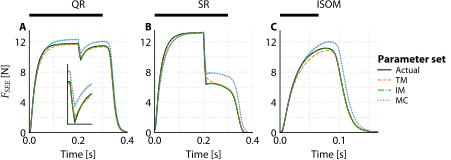
\includegraphics[keepaspectratio]{../figures/r_protocols.pdf}}

}

\caption{\label{fig-r-protocols}\textbf{Representative example of SEE
force over time during a quick-release (A), step-ramp (B) and isometric
experiment (C).} The inset in (A) depicts the SEE force over time around
the quick-release. The SEE force over time is depicted for four sets of
parameter values: 1) the actual values (i.e., literature-obtained; black
solid line), those obtained with the traditional method (TM; orange
dashed line), those obtained with the improved method (IM; green
dashed-dotted line) and those resulting from the Monte Carlo Simulations
(MC; blue dotted line, with shaded 95\% confidence interval).}

\end{figure}%

\begin{table}[h]

\caption{\label{tbl-r-pdiff}Percentage differences between estimated and
actual MTC parameter values.}

\centering{

%\begin{tabular}{|l|c|c|c|c|c|c|c|c|c|} \hline
 & \multicolumn{3}{c|}{\itshape Traditional method} & \multicolumn{3}{c|}{\itshape Improved method} & \multicolumn{3}{c|}{\itshape Monte Carlo} \\ \hline
 & \bfseries GM1 & \bfseries GM2 & \bfseries GM3 & \bfseries GM1 & \bfseries GM2 & \bfseries GM3 & \bfseries GM1 & \bfseries GM2 & \bfseries GM3 \\ \hline
$a$ &  1 &  4 &  2 &  1 &  3 &  1 &  1 ±  2 &  6 ±  2 &  1 ±  2 \\ \hline
$b$ & -0 &  2 & -1 &  1 &  2 &  1 &  1 ±  2 &  5 ±  2 &  1 ±  2 \\ \hline
$F_{CE}^{max}$ &  0 & -1 &  0 & -0 & -1 & -0 & -0 ±  1 & -2 ±  1 & -0 ±  1 \\ \hline
$k_{PEE}$ &  3 & -9 &  9 & -0 &  0 & -0 &  3 ± 17 &  3 ± 16 &  6 ± 31 \\ \hline
$k_{SEE}$ & -39 & -27 & -37 &  0 & -1 &  0 & -37 ±  6 & -36 ±  6 & -36 ±  6 \\ \hline
$L_{CE}^{opt}$ & -1 & -2 & -3 & -0 &  0 & -0 &  0 ±  3 &  0 ±  2 &  0 ±  3 \\ \hline
$L_{PEE}^0$ &  0 & -1 & -0 & -0 &  0 & -0 &  0 ±  3 &  1 ±  2 &  0 ±  2 \\ \hline
$L_{SEE}^0$ & -1 & -0 & -0 &  0 & -0 &  0 & -0 ±  1 & -0 ±  1 & -0 ±  1 \\ \hline
$\tau_{act}$ & -21 & -16 & -21 & -0 & -1 & -0 &  1 ±  3 & -0 ±  4 &  1 ±  4 \\ \hline
$\tau_{deact}$ & -5 & -4 & -5 &  0 &  0 &  0 &  0 ±  1 &  0 ±  1 &  0 ±  1 \\ \hline
\end{tabular}

}

\end{table}%

\subsubsection{Understanding errors in parameter value
estimation}\label{understanding-errors-in-parameter-value-estimation}

\textbf{Estimation of SEE stiffness.} The SEE stiffness parameter
(\(k_{SEE}\)) was underestimated by 39\%, 27\% and 37\% for GM1, GM2 and
GM3, respectively (see Table~\ref{tbl-r-pdiff}). This overestimation
directly resulted from the overestimation of SEE shortening due to the
quick-release, which was overestimated by 28±2\%, 17±2\% and 26±2\% for
GM1, GM2 and GM3, respectively, averaged across all quick-release
experiments. In absolute terms, CE shortened only 43±3, 29±2 and 41±2 µm
over the 11\,ms interval between the time points at which SEE force and
SEE length were sampled (i.e., immediately before and after the
quick-release). The amount of CE shortening was smallest in GM2 because
GM2 was a slower muscle than GM1 and GM3. Consequently, the
overestimation of SEE shortening was also smallest in GM2, which in turn
led to the smallest underestimation of \(k_{SEE}\). All in all, this
shows that even very small amounts of CE shortening has substantial
influence on the estimation of SEE stiffness.

Since SEE was very stiff, the overestimation in SEE elongation at
maximal isometric CE force was only 0.50, 0.32 and 0.49 mm for GM1, GM2
and GM3, respectively. This is an important finding because the SEE
stiffness is the first parameter in the estimation process and therefore
affects all subsequent estimated parameter values. Therefore, since the
overestimation of SEE elongation (in mm) at maximal isometric CE force
was only small, the impact on the estimation of the other contraction
dynamics parameter values was also small.

Lastly, it should be noted that the correlation coefficient between the
data SEE force‑length relationship and the one based from the estimated
parameters is not an adequate measure of how accurately SEE stiffness is
captured. Obviously, a correlation coefficient is not sensitive to the
overestimation of SEE shortening due to the quick-release. Consequently,
high correlation coefficients (\(R^2 >\) 0.99) can still be observed
even when SEE stiffness is substantially underestimated. To further
investigate this issue, we simulated the quick-release experiments after
obtaining all contraction and excitation dynamics parameter values. The
simulations clearly showed a slower rise in SEE force after the
quick-release in comparison with the experimental data
(Figure~\ref{fig-r-protocols}A), indicating that SEE stiffness was
underestimated. These results suggest that the rise in SEE force is a
better measure of SEE stiffness estimation accuracy.

\subsection{Sensitivity analysis}\label{sensitivity-analysis}

\begin{Shaded}
\begin{Highlighting}[]
\CommentTok{\# \%\% Load packages}
\ImportTok{import}\NormalTok{ os, pickle, sys}
\ImportTok{import}\NormalTok{ pandas }\ImportTok{as}\NormalTok{ pd}
\ImportTok{from}\NormalTok{ pathlib }\ImportTok{import}\NormalTok{ Path}

\CommentTok{\# Set directories}
\NormalTok{cwd }\OperatorTok{=}\NormalTok{ Path.cwd()}
\NormalTok{baseDir }\OperatorTok{=}\NormalTok{ cwd.parent}
\NormalTok{dataDir }\OperatorTok{=}\NormalTok{ baseDir }\OperatorTok{/} \StringTok{\textquotesingle{}data\textquotesingle{}}
\NormalTok{funcDir }\OperatorTok{=}\NormalTok{ baseDir }\OperatorTok{/} \StringTok{\textquotesingle{}analysis\textquotesingle{}} \OperatorTok{/} \StringTok{\textquotesingle{}functions\textquotesingle{}}
\NormalTok{sys.path.append(}\BuiltInTok{str}\NormalTok{(funcDir))}

\CommentTok{\# Custom functions}
\ImportTok{import}\NormalTok{ stats}

\CommentTok{\# \%\% 3.2.1: Monte Carlo simulations}
\NormalTok{muscles }\OperatorTok{=}\NormalTok{ [}\StringTok{\textquotesingle{}GMs1\textquotesingle{}}\NormalTok{, }\StringTok{\textquotesingle{}GMs2\textquotesingle{}}\NormalTok{, }\StringTok{\textquotesingle{}GMs3\textquotesingle{}}\NormalTok{]}
\CommentTok{\# Parameters to track}
\NormalTok{params }\OperatorTok{=}\NormalTok{ [}\StringTok{\textquotesingle{}a\textquotesingle{}}\NormalTok{, }\StringTok{\textquotesingle{}b\textquotesingle{}}\NormalTok{, }\StringTok{\textquotesingle{}fmax\textquotesingle{}}\NormalTok{, }\StringTok{\textquotesingle{}kpee\textquotesingle{}}\NormalTok{, }\StringTok{\textquotesingle{}ksee\textquotesingle{}}\NormalTok{, }\StringTok{\textquotesingle{}lce\_opt\textquotesingle{}}\NormalTok{, }\StringTok{\textquotesingle{}lpee0\textquotesingle{}}\NormalTok{, }\StringTok{\textquotesingle{}lsee0\textquotesingle{}}\NormalTok{, }\StringTok{\textquotesingle{}tact\textquotesingle{}}\NormalTok{, }\StringTok{\textquotesingle{}tdeact\textquotesingle{}}\NormalTok{]}

\CommentTok{\# Store Monte{-}Carlo results}
\NormalTok{results }\OperatorTok{=}\NormalTok{ []}
\ControlFlowTok{for}\NormalTok{ mus }\KeywordTok{in}\NormalTok{ muscles:}
\NormalTok{    par\_file }\OperatorTok{=}\NormalTok{ os.path.join(dataDir, mus, }\StringTok{\textquotesingle{}parameters\textquotesingle{}}\NormalTok{, }\SpecialStringTok{f\textquotesingle{}}\SpecialCharTok{\{}\NormalTok{mus}\SpecialCharTok{\}}\SpecialStringTok{\_OR.pkl\textquotesingle{}}\NormalTok{)}
\NormalTok{    or\_par }\OperatorTok{=}\NormalTok{ pickle.load(}\BuiltInTok{open}\NormalTok{(par\_file, }\StringTok{\textquotesingle{}rb\textquotesingle{}}\NormalTok{))}
\NormalTok{    eseeMaxOR }\OperatorTok{=}\NormalTok{ (or\_par[}\StringTok{\textquotesingle{}fmax\textquotesingle{}}\NormalTok{]}\OperatorTok{/}\NormalTok{or\_par[}\StringTok{\textquotesingle{}ksee\textquotesingle{}}\NormalTok{])}\OperatorTok{**}\FloatTok{0.5}
        
    
    \ControlFlowTok{for}\NormalTok{ iMC }\KeywordTok{in} \BuiltInTok{range}\NormalTok{(}\DecValTok{1}\NormalTok{, }\DecValTok{51}\NormalTok{):}
\NormalTok{        mc\_file }\OperatorTok{=}\NormalTok{ os.path.join(dataDir, mus, }\StringTok{\textquotesingle{}parameters\textquotesingle{}}\NormalTok{,}\StringTok{\textquotesingle{}mc\textquotesingle{}}\NormalTok{, }\SpecialStringTok{f\textquotesingle{}}\SpecialCharTok{\{}\NormalTok{mus}\SpecialCharTok{\}}\SpecialStringTok{\_MC}\SpecialCharTok{\{}\NormalTok{iMC}\SpecialCharTok{:02d\}}\SpecialStringTok{.pkl\textquotesingle{}}\NormalTok{)}
\NormalTok{        mc\_par }\OperatorTok{=}\NormalTok{ pickle.load(}\BuiltInTok{open}\NormalTok{(mc\_file, }\StringTok{\textquotesingle{}rb\textquotesingle{}}\NormalTok{))[}\DecValTok{0}\NormalTok{]}
\NormalTok{        eseeMaxMC }\OperatorTok{=}\NormalTok{ (mc\_par[}\StringTok{\textquotesingle{}fmax\textquotesingle{}}\NormalTok{]}\OperatorTok{/}\NormalTok{mc\_par[}\StringTok{\textquotesingle{}ksee\textquotesingle{}}\NormalTok{])}\OperatorTok{**}\FloatTok{0.5}
        
\NormalTok{        entry }\OperatorTok{=}\NormalTok{ \{}\StringTok{\textquotesingle{}muscle\textquotesingle{}}\NormalTok{: mus, }\StringTok{\textquotesingle{}MC\textquotesingle{}}\NormalTok{: iMC, }\StringTok{\textquotesingle{}d\_esee\textquotesingle{}}\NormalTok{: (eseeMaxMC}\OperatorTok{{-}}\NormalTok{eseeMaxOR)\}}
        \ControlFlowTok{for}\NormalTok{ param }\KeywordTok{in}\NormalTok{ params:}
\NormalTok{            entry[param] }\OperatorTok{=}\NormalTok{ stats.pdiff(mc\_par[param], or\_par[param])}
        
\NormalTok{        results.append(entry)}

\CommentTok{\# Convert to pandas DataFrame}
\NormalTok{df }\OperatorTok{=}\NormalTok{ pd.DataFrame(results)}

\CommentTok{\# Compute summary statistics}
\NormalTok{df\_mean }\OperatorTok{=}\NormalTok{ df.groupby(}\StringTok{\textquotesingle{}muscle\textquotesingle{}}\NormalTok{).mean().T}
\NormalTok{df\_std }\OperatorTok{=}\NormalTok{ df.groupby(}\StringTok{\textquotesingle{}muscle\textquotesingle{}}\NormalTok{).std().T}

\CommentTok{\# Extract all contraction dynamics parameters except ksee}
\NormalTok{p\_MC\_con\_avg }\OperatorTok{=}\NormalTok{ df\_mean.loc[[}\StringTok{\textquotesingle{}a\textquotesingle{}}\NormalTok{,}\StringTok{\textquotesingle{}b\textquotesingle{}}\NormalTok{, }\StringTok{\textquotesingle{}kpee\textquotesingle{}}\NormalTok{, }\StringTok{\textquotesingle{}fmax\textquotesingle{}}\NormalTok{, }\StringTok{\textquotesingle{}lce\_opt\textquotesingle{}}\NormalTok{, }\StringTok{\textquotesingle{}lpee0\textquotesingle{}}\NormalTok{, }\StringTok{\textquotesingle{}lsee0\textquotesingle{}}\NormalTok{]]}
\NormalTok{p\_MC\_con\_std }\OperatorTok{=}\NormalTok{ df\_std.loc[[}\StringTok{\textquotesingle{}a\textquotesingle{}}\NormalTok{, }\StringTok{\textquotesingle{}b\textquotesingle{}}\NormalTok{, }\StringTok{\textquotesingle{}fmax\textquotesingle{}}\NormalTok{, }\StringTok{\textquotesingle{}kpee\textquotesingle{}}\NormalTok{, }\StringTok{\textquotesingle{}lce\_opt\textquotesingle{}}\NormalTok{, }\StringTok{\textquotesingle{}lpee0\textquotesingle{}}\NormalTok{, }\StringTok{\textquotesingle{}lsee0\textquotesingle{}}\NormalTok{]]}

\CommentTok{\# Percentage difference over all muscles: from real to estimated ksee}
\NormalTok{p\_MC\_ksee\_avg }\OperatorTok{=} \SpecialStringTok{f\textquotesingle{}}\SpecialCharTok{\{}\NormalTok{df\_mean}\SpecialCharTok{.}\NormalTok{loc[}\StringTok{\textquotesingle{}ksee\textquotesingle{}}\NormalTok{]}\SpecialCharTok{.}\NormalTok{mean()}\SpecialCharTok{:0.0f\}}\SpecialStringTok{\textquotesingle{}}  \CommentTok{\# [\%] percentage difference}
\CommentTok{\# Absolute difference over all muscles of SEE elongation @ Fcemax}
\NormalTok{d\_MC\_esee\_avg }\OperatorTok{=} \SpecialStringTok{f\textquotesingle{}}\SpecialCharTok{\{}\NormalTok{df\_mean}\SpecialCharTok{.}\NormalTok{loc[}\StringTok{\textquotesingle{}d\_esee\textquotesingle{}}\NormalTok{]}\SpecialCharTok{.}\NormalTok{mean()}\OperatorTok{*}\FloatTok{1e3}\SpecialCharTok{:0.1f\}}\SpecialStringTok{\textquotesingle{}}  \CommentTok{\# [mm]}
\CommentTok{\# Max. avg. percentage difference over all muscles: from real to estimated value of contraction dyn. parms}
\NormalTok{p\_MC\_con\_maxavg }\OperatorTok{=} \SpecialStringTok{f\textquotesingle{}}\SpecialCharTok{\{}\NormalTok{p\_MC\_con\_avg}\SpecialCharTok{.}\BuiltInTok{abs}\NormalTok{()}\SpecialCharTok{.}\BuiltInTok{max}\NormalTok{()}\SpecialCharTok{.}\BuiltInTok{max}\NormalTok{()}\SpecialCharTok{:0.1f\}}\SpecialStringTok{\textquotesingle{}} 
\CommentTok{\# Max. std. percentage difference over all muscles: from real to estimated value of contraction dyn. parms}
\NormalTok{p\_MC\_con\_maxstd }\OperatorTok{=} \SpecialStringTok{f\textquotesingle{}}\SpecialCharTok{\{}\NormalTok{p\_MC\_con\_std}\SpecialCharTok{.}\BuiltInTok{abs}\NormalTok{()}\SpecialCharTok{.}\BuiltInTok{max}\NormalTok{()}\SpecialCharTok{.}\BuiltInTok{max}\NormalTok{()}\SpecialCharTok{:0.0f\}}\SpecialStringTok{\textquotesingle{}} 
\CommentTok{\# Max. std percentage difference over all muscles: from real to estimated value of kpee}
\NormalTok{p\_MC\_kpee\_maxstd }\OperatorTok{=} \SpecialStringTok{f\textquotesingle{}}\SpecialCharTok{\{}\NormalTok{df\_std}\SpecialCharTok{.}\NormalTok{loc[}\StringTok{\textquotesingle{}kpee\textquotesingle{}}\NormalTok{]}\SpecialCharTok{.}\BuiltInTok{max}\NormalTok{()}\SpecialCharTok{:0.0f\}}\SpecialStringTok{\textquotesingle{}}
\CommentTok{\# Max. avg percentage difference over all muscles: from real to estimated value of tact}
\NormalTok{p\_MC\_tact\_maxavg }\OperatorTok{=} \SpecialStringTok{f\textquotesingle{}}\SpecialCharTok{\{}\NormalTok{df\_mean}\SpecialCharTok{.}\NormalTok{loc[}\StringTok{\textquotesingle{}tact\textquotesingle{}}\NormalTok{]}\SpecialCharTok{.}\BuiltInTok{max}\NormalTok{()}\SpecialCharTok{:0.1f\}}\SpecialStringTok{\textquotesingle{}}
\CommentTok{\# Avg. std percentage difference over all muscles: from real to estimated value of tact}
\NormalTok{p\_MC\_tact\_avgstd }\OperatorTok{=} \SpecialStringTok{f\textquotesingle{}}\SpecialCharTok{\{}\NormalTok{df\_std}\SpecialCharTok{.}\NormalTok{loc[}\StringTok{\textquotesingle{}tact\textquotesingle{}}\NormalTok{]}\SpecialCharTok{.}\NormalTok{mean()}\SpecialCharTok{:0.0f\}}\SpecialStringTok{\textquotesingle{}}
\end{Highlighting}
\end{Shaded}

\subsubsection{Monte Carlo simulations}\label{monte-carlo-simulations-1}

Monte Carlo simulations were used to examine how shifts in the MTC
force--length relationship caused by a decrease in SEE stiffness (e.g.,
due to irreversible SEE damage in experiments) affect the accuracy of
the estimated contraction and excitation dynamics parameter values. The
induced shifts of the MTC force-length relationship were between 0--1
mm, and therefore it was no surprise that SEE stiffness decreased by
36\% on average --- which corresponds to a .5 mm shift.

All other estimated contraction dynamics parameter values were within
6.3\% on average of their actual value (Table~\ref{tbl-r-pdiff}). The
variance in the estimated contraction dynamics parameter values was
below 31\% for all parameters except for the PEE stiffness scaling
parameter. The PEE stiffness scaling parameter showed substantially
higher variance (with a standard deviation up to 31\%), because it was
based on four or fewer quick-release trials, making it more sensitive to
perturbations in the data. Regarding the excitation dynamics, the
influence on the average time constants was minimal (within 0.7\%), but
affected the variance in the estimated values of the activation time
constant (with a standard deviation of 4\% on average). These findings
indicate that an average decrease in SEE stiffness of 36\% has a much
smaller effect on the estimated parameter values of the contraction and
excitation dynamics, even at the level of an individual muscle.

\subsubsection{Interdependency of parameter
values}\label{interdependency-of-parameter-values-1}

We investigated the interdependency of the estimated parameter values by
adjusting each parameter value by 5\% and re-estimating all other
parameter values. \(F_{CE}^{max}\) and \(L_{SEE}^0\) were the parameters
that had most effect on the estimates of the others.

First, \(F_{CE}^{max}\) affected the estimation of parameter \(a\) and
\(b\) of the CE force-velocity relationship. Underestimating
\(F_{CE}^{max}\) leads to an underestimation of CE force at 0 velocity.
Due to the formulation of the CE force-velocity relationship, the curve,
by definition, crosses the point at \(v_{CE}=0\) and
\(F_{CE}=F_{CE}^{max}\). Consequently, the best fit to the data with an
underestimated \(F_{CE}^{max}\) is a much flatter CE force-velocity
relationship, which is realised by an increase in \(a\) and a decrease
in \(b\). This flatter CE force-velocity relationship affects the
estimation of all other contraction dynamics parameter values because
the CE force-velocity relationship is used to estimate the CE shortening
due to the quick-release (see Section~\ref{sec-m-im}). As a result,
\(k_{SEE}\) and \(L_{SEE}^0\) decreased due to underestimating
\(F_{CE}^{max}\), whereas \(L_{CE}^{opt}\) increased. In summary,
\(F_{CE}^{max}\) substantially influenced the estimation of all
contraction dynamics parameter values mainly by its effect on the CE
force-velocity relationship.

Second, \(L_{SEE}^0\) affected the estimation of \(L_{CE}^{opt}\) and
\(F_{CE}^{max}\). As explained earlier, when \(L_{SEE}^0\) is
overestimated, \(L_{CE}^{opt}\) is underestimated, such that
\(L_{MTC}^{opt}\) remains more or less unaffected. Underestimating
\(L_{CE}^{opt}\) causes a narrower MTC force-length relationship,
leading to an overestimation of \(F_{CE}^{max}\) to preserve a good fit
between the data and the model. As previously discussed, overestimating
\(F_{CE}^{max}\), in turn, resulted in an underestimation of parameters
\(a\) and \(b\). Thus, \(L_{SEE}^0\) substantially influenced the
estimation of all contraction dynamics parameter values mainly by its
effect on the MTC force-length relationship.

Taken together, the interdependence of \(F_{CE}^{max}\) and
\(L_{SEE}^0\) with other parameter values underscores the need for
precise estimation of these key parameters. In this regard, it is
reassuring that these two parameters were found to be robust for
perturbations in the experimental data.

\begin{table}[h]

\caption{\label{tbl-r-interdep}Interdependency of the estimated MTC
parameter values. Each entry shows the percentage change in the row
parameter resulting from a 5\% change in the column parameter. All
values are expressed as percentage changes.}

\centering{

%\begin{tabular}{|l|c|c|c|c|c|c|} \hline
 & $\mathbold{a}$ & $\mathbold{b}$ & $\mathbold{F_{CE}^{max}}$ & $\mathbold{k_{SEE}}$ & $\mathbold{L_{CE}^{opt}}$ & $\mathbold{L_{SEE}^{0}}$ \\ \hline
$a$ & - & 10.1 ± 1.3 & -14.0 ± 1.0 & -0.6 ± 0.2 & 3.4 ± 1.0 & -10.3 ± 2.0 \\ \hline
$b$ & 2.3 ± 1.2 & - & -14.3 ± 3.1 & 1.1 ± 0.3 & 3.9 ± 1.1 & -10.8 ± 1.6 \\ \hline
$F_{CE}^{max}$ & -0.6 ± 0.1 & -0.6 ± 0.1 & - & -0.6 ± 0.2 & -1.2 ± 0.5 & 3.5 ± 0.5 \\ \hline
$k_{PEE}$ & -6.8 ± 2.9 & -6.8 ± 2.9 & -6.9 ± 3.5 & -6.8 ± 3.2 & -6.8 ± 2.9 & -6.8 ± 3.3 \\ \hline
$k_{SEE}$ & 52.4 ± 12.6 & 52.4 ± 12.8 & 54.3 ± 17.0 & - & 52.4 ± 12.8 & 52.5 ± 14.3 \\ \hline
$L_{CE}^{opt}$ & 1.9 ± 0.6 & 1.9 ± 0.6 & -5.4 ± 2.2 & 1.9 ± 0.6 & - & -14.2 ± 3.0 \\ \hline
$L_{PEE}^0$ & -0.6 ± 0.7 & -0.6 ± 0.7 & -0.6 ± 0.7 & -0.6 ± 0.7 & -0.6 ± 0.7 & -10.6 ± 1.2 \\ \hline
$L_{SEE}^0$ & 0.5 ± 0.2 & 0.5 ± 0.2 & 1.8 ± 0.6 & 0.5 ± 0.2 & -1.7 ± 0.6 & - \\ \hline
$\tau_{act}$ & 23.4 ± 4.2 & 23.4 ± 4.6 & 24.2 ± 5.9 & 23.3 ± 5.0 & 23.7 ± 4.3 & 20.9 ± 6.3 \\ \hline
$\tau_{deact}$ & 4.8 ± 0.7 & 4.9 ± 0.8 & 5.0 ± 3.1 & 4.8 ± 0.9 & 4.9 ± 1.4 & 5.1 ± 3.0 \\ \hline
\end{tabular}

}

\end{table}%

\subsection{\texorpdfstring{Evaluating model predictions - \emph{in
situ}
data}{Evaluating model predictions - in situ data}}\label{evaluating-model-predictions---in-situ-data}

\begin{Shaded}
\begin{Highlighting}[]
\CommentTok{\# \%\% Load packages}
\ImportTok{import}\NormalTok{ os, pickle, sys, glob}
\ImportTok{import}\NormalTok{ numpy }\ImportTok{as}\NormalTok{ np}
\ImportTok{import}\NormalTok{ pandas }\ImportTok{as}\NormalTok{ pd}
\ImportTok{from}\NormalTok{ pathlib }\ImportTok{import}\NormalTok{ Path}

\CommentTok{\# Directories}
\NormalTok{cwd }\OperatorTok{=}\NormalTok{ Path.cwd()}
\NormalTok{baseDir }\OperatorTok{=}\NormalTok{ cwd.parent}
\NormalTok{dataDir }\OperatorTok{=}\NormalTok{ baseDir }\OperatorTok{/} \StringTok{\textquotesingle{}data\textquotesingle{}}
\NormalTok{funcDir }\OperatorTok{=}\NormalTok{ baseDir }\OperatorTok{/} \StringTok{\textquotesingle{}analysis\textquotesingle{}} \OperatorTok{/} \StringTok{\textquotesingle{}functions\textquotesingle{}}
\NormalTok{sys.path.append(}\BuiltInTok{str}\NormalTok{(funcDir))}

\CommentTok{\# Custom functions}
\ImportTok{import}\NormalTok{ helpers, stats}

\CommentTok{\# \%\% Extract parameters}
\NormalTok{muscles }\OperatorTok{=}\NormalTok{ [}\StringTok{\textquotesingle{}GMe1\textquotesingle{}}\NormalTok{, }\StringTok{\textquotesingle{}GMe2\textquotesingle{}}\NormalTok{, }\StringTok{\textquotesingle{}GMe3\textquotesingle{}}\NormalTok{]}
\NormalTok{param\_keys }\OperatorTok{=}\NormalTok{ [}\StringTok{\textquotesingle{}a\textquotesingle{}}\NormalTok{, }\StringTok{\textquotesingle{}b\textquotesingle{}}\NormalTok{, }\StringTok{\textquotesingle{}kpee\textquotesingle{}}\NormalTok{, }\StringTok{\textquotesingle{}ksee\textquotesingle{}}\NormalTok{, }\StringTok{\textquotesingle{}fmax\textquotesingle{}}\NormalTok{, }\StringTok{\textquotesingle{}lce\_opt\textquotesingle{}}\NormalTok{, }\StringTok{\textquotesingle{}lpee0\textquotesingle{}}\NormalTok{, }\StringTok{\textquotesingle{}lsee0\textquotesingle{}}\NormalTok{, }\StringTok{\textquotesingle{}tact\textquotesingle{}}\NormalTok{, }\StringTok{\textquotesingle{}tdeact\textquotesingle{}}\NormalTok{]}

\NormalTok{orParms, tmParms, imParms }\OperatorTok{=}\NormalTok{ [], [], []}
\ControlFlowTok{for}\NormalTok{ mus }\KeywordTok{in}\NormalTok{ muscles:   }
\NormalTok{    tmPar, dataQRtm }\OperatorTok{=}\NormalTok{ pickle.load(}\BuiltInTok{open}\NormalTok{(os.path.join(dataDir,mus,}\StringTok{\textquotesingle{}parameters\textquotesingle{}}\NormalTok{,mus}\OperatorTok{+}\StringTok{\textquotesingle{}\_TM.pkl\textquotesingle{}}\NormalTok{), }\StringTok{\textquotesingle{}rb\textquotesingle{}}\NormalTok{))[}\DecValTok{0}\NormalTok{:}\DecValTok{2}\NormalTok{]}
\NormalTok{    imPar, dataQRim }\OperatorTok{=}\NormalTok{ pickle.load(}\BuiltInTok{open}\NormalTok{(os.path.join(dataDir,mus,}\StringTok{\textquotesingle{}parameters\textquotesingle{}}\NormalTok{,mus}\OperatorTok{+}\StringTok{\textquotesingle{}\_IM.pkl\textquotesingle{}}\NormalTok{), }\StringTok{\textquotesingle{}rb\textquotesingle{}}\NormalTok{))[}\DecValTok{0}\NormalTok{:}\DecValTok{2}\NormalTok{]}
    
\NormalTok{    parms }\OperatorTok{=}\NormalTok{ [tmPar[k] }\ControlFlowTok{for}\NormalTok{ k }\KeywordTok{in}\NormalTok{ param\_keys]}
\NormalTok{    tmParms.append(parms)}
    
\NormalTok{    parms }\OperatorTok{=}\NormalTok{ [imPar[k] }\ControlFlowTok{for}\NormalTok{ k }\KeywordTok{in}\NormalTok{ param\_keys]}
\NormalTok{    imParms.append(parms)}
    
\CommentTok{\# Store in pandas dataframe}
\NormalTok{df\_tm }\OperatorTok{=}\NormalTok{ pd.DataFrame(}\BuiltInTok{list}\NormalTok{(}\BuiltInTok{zip}\NormalTok{(}\OperatorTok{*}\NormalTok{tmParms)), columns}\OperatorTok{=}\NormalTok{[}\StringTok{\textquotesingle{}GM1\textquotesingle{}}\NormalTok{, }\StringTok{\textquotesingle{}GM2\textquotesingle{}}\NormalTok{, }\StringTok{\textquotesingle{}GM3\textquotesingle{}}\NormalTok{], index}\OperatorTok{=}\NormalTok{param\_keys) }\CommentTok{\# df with estimated parameter values using the traditional method}
\NormalTok{df\_im }\OperatorTok{=}\NormalTok{ pd.DataFrame(}\BuiltInTok{list}\NormalTok{(}\BuiltInTok{zip}\NormalTok{(}\OperatorTok{*}\NormalTok{imParms)), columns}\OperatorTok{=}\NormalTok{[}\StringTok{\textquotesingle{}GM1\textquotesingle{}}\NormalTok{, }\StringTok{\textquotesingle{}GM2\textquotesingle{}}\NormalTok{, }\StringTok{\textquotesingle{}GM3\textquotesingle{}}\NormalTok{], index}\OperatorTok{=}\NormalTok{param\_keys) }\CommentTok{\# df with estimated parameter values using the improved method}

\CommentTok{\# \%\% Compute percentage differences from real/actual and estimated parameter values}
\CommentTok{\# Positive: Imporoved is that \% higher than Traditional}
\CommentTok{\# Negative: Imporoved is that \% lower than Traditional}
\NormalTok{df\_p }\OperatorTok{=}\NormalTok{ stats.pdiff(df\_im, df\_tm)}

\CommentTok{\# \%\% Compute RMSDs}
\NormalTok{par\_models }\OperatorTok{=}\NormalTok{ [}\StringTok{\textquotesingle{}TM\textquotesingle{}}\NormalTok{, }\StringTok{\textquotesingle{}IM\textquotesingle{}}\NormalTok{]}
\NormalTok{experiments }\OperatorTok{=}\NormalTok{ [}\StringTok{\textquotesingle{}QR\textquotesingle{}}\NormalTok{, }\StringTok{\textquotesingle{}SR\textquotesingle{}}\NormalTok{, }\StringTok{\textquotesingle{}ISOM\textquotesingle{}}\NormalTok{, }\StringTok{\textquotesingle{}SSC\textquotesingle{}}\NormalTok{]}
\NormalTok{muscles }\OperatorTok{=}\NormalTok{ [}\StringTok{\textquotesingle{}GMe1\textquotesingle{}}\NormalTok{, }\StringTok{\textquotesingle{}GMe2\textquotesingle{}}\NormalTok{, }\StringTok{\textquotesingle{}GMe3\textquotesingle{}}\NormalTok{]}

\NormalTok{avg\_mean\_all }\OperatorTok{=}\NormalTok{ []}
\NormalTok{columns }\OperatorTok{=}\NormalTok{ [}\SpecialStringTok{f\textquotesingle{}}\SpecialCharTok{\{}\NormalTok{model}\SpecialCharTok{\}}\SpecialStringTok{\_}\SpecialCharTok{\{}\NormalTok{exp}\SpecialCharTok{\}}\SpecialStringTok{\textquotesingle{}} \ControlFlowTok{for}\NormalTok{ model }\KeywordTok{in}\NormalTok{ par\_models }\ControlFlowTok{for}\NormalTok{ exp }\KeywordTok{in}\NormalTok{ experiments]}
\NormalTok{rows }\OperatorTok{=}\NormalTok{ muscles }\OperatorTok{+}\NormalTok{ [}\StringTok{\textquotesingle{}Avg ± Std\textquotesingle{}}\NormalTok{]}
\NormalTok{df }\OperatorTok{=}\NormalTok{ pd.DataFrame(index}\OperatorTok{=}\NormalTok{rows, columns}\OperatorTok{=}\NormalTok{columns, dtype}\OperatorTok{=}\BuiltInTok{str}\NormalTok{)}
\ControlFlowTok{for}\NormalTok{ exp }\KeywordTok{in}\NormalTok{ experiments:}
    \ControlFlowTok{for}\NormalTok{ model }\KeywordTok{in}\NormalTok{ par\_models:}
\NormalTok{        all\_rmsd }\OperatorTok{=}\NormalTok{ []}
        \ControlFlowTok{for}\NormalTok{ mus }\KeywordTok{in}\NormalTok{ muscles:}
            \CommentTok{\# Load parameter}
\NormalTok{            parFile }\OperatorTok{=}\NormalTok{ os.path.join(dataDir, mus, }\StringTok{\textquotesingle{}parameters\textquotesingle{}}\NormalTok{, }\SpecialStringTok{f\textquotesingle{}}\SpecialCharTok{\{}\NormalTok{mus}\SpecialCharTok{\}}\SpecialStringTok{\_}\SpecialCharTok{\{}\NormalTok{model}\SpecialCharTok{\}}\SpecialStringTok{.pkl\textquotesingle{}}\NormalTok{)}
\NormalTok{            muspar }\OperatorTok{=}\NormalTok{ pickle.load(}\BuiltInTok{open}\NormalTok{(parFile, }\StringTok{\textquotesingle{}rb\textquotesingle{}}\NormalTok{))[}\DecValTok{0}\NormalTok{]}

\NormalTok{            dataDirExp }\OperatorTok{=}\NormalTok{ os.path.join(dataDir, mus, }\StringTok{\textquotesingle{}dataExp\textquotesingle{}}\NormalTok{, exp)}
\NormalTok{            rrunDirExp }\OperatorTok{=}\NormalTok{ os.path.join(dataDir, mus, }\StringTok{\textquotesingle{}simsExp\textquotesingle{}}\NormalTok{, model, exp)}

\NormalTok{            dataFiles }\OperatorTok{=} \BuiltInTok{sorted}\NormalTok{(glob.glob(os.path.join(dataDirExp, }\StringTok{\textquotesingle{}*\textquotesingle{}}\NormalTok{)))}
\NormalTok{            rrunFiles }\OperatorTok{=} \BuiltInTok{sorted}\NormalTok{(glob.glob(os.path.join(rrunDirExp, }\StringTok{\textquotesingle{}*\textquotesingle{}}\NormalTok{)))}

\NormalTok{            rms\_list }\OperatorTok{=}\NormalTok{ []}
            \ControlFlowTok{for}\NormalTok{ dataFile, rrunFile }\KeywordTok{in} \BuiltInTok{zip}\NormalTok{(dataFiles, rrunFiles):}
\NormalTok{                dataFilename }\OperatorTok{=}\NormalTok{ os.path.basename(dataFile)[:}\OperatorTok{{-}}\DecValTok{4}\NormalTok{]}
\NormalTok{                rrunFilename }\OperatorTok{=}\NormalTok{ os.path.basename(rrunFile)[:}\OperatorTok{{-}}\DecValTok{4}\NormalTok{]}
                \ControlFlowTok{if}\NormalTok{ dataFilename[:}\OperatorTok{{-}}\DecValTok{3}\NormalTok{] }\OperatorTok{!=}\NormalTok{ rrunFilename[:}\OperatorTok{{-}}\DecValTok{3}\NormalTok{]:}
                    \ControlFlowTok{raise} \PreprocessorTok{ValueError}\NormalTok{(}\SpecialStringTok{f"File mismatch: }\SpecialCharTok{\{}\NormalTok{dataFilename}\SpecialCharTok{\}}\SpecialStringTok{ vs }\SpecialCharTok{\{}\NormalTok{rrunFilename}\SpecialCharTok{\}}\SpecialStringTok{"}\NormalTok{)}

\NormalTok{                dataData }\OperatorTok{=}\NormalTok{ pd.read\_csv(dataFile).T.to\_numpy()[}\DecValTok{0}\NormalTok{:}\DecValTok{4}\NormalTok{]}
\NormalTok{                rrunData }\OperatorTok{=}\NormalTok{ pd.read\_csv(rrunFile).T.to\_numpy()}

\NormalTok{                time1, \_, stim1, fsee1 }\OperatorTok{=}\NormalTok{ dataData}
\NormalTok{                time2, \_, \_, fsee2 }\OperatorTok{=}\NormalTok{ rrunData}

\NormalTok{                tStimOn, tStimOff }\OperatorTok{=}\NormalTok{ helpers.get\_stim(time1, stim1)[}\DecValTok{1}\NormalTok{:]}
\NormalTok{                iStart }\OperatorTok{=} \BuiltInTok{int}\NormalTok{(np.argmin(}\BuiltInTok{abs}\NormalTok{(time1 }\OperatorTok{{-}}\NormalTok{ tStimOn[}\DecValTok{0}\NormalTok{])))}

                \ControlFlowTok{if}\NormalTok{ exp }\OperatorTok{==} \StringTok{\textquotesingle{}ISOM\textquotesingle{}}\NormalTok{:}
\NormalTok{                    iStop }\OperatorTok{=} \BuiltInTok{int}\NormalTok{(np.argmin(}\BuiltInTok{abs}\NormalTok{(time1 }\OperatorTok{{-}} \FloatTok{0.1} \OperatorTok{{-}}\NormalTok{ tStimOff[}\DecValTok{0}\NormalTok{])))}
                \ControlFlowTok{elif}\NormalTok{ exp }\KeywordTok{in}\NormalTok{ [}\StringTok{\textquotesingle{}QR\textquotesingle{}}\NormalTok{, }\StringTok{\textquotesingle{}SR\textquotesingle{}}\NormalTok{]:}
\NormalTok{                    iStop }\OperatorTok{=} \BuiltInTok{int}\NormalTok{(np.argmin(}\BuiltInTok{abs}\NormalTok{(time1 }\OperatorTok{{-}}\NormalTok{ tStimOff[}\DecValTok{0}\NormalTok{])))}
                \ControlFlowTok{else}\NormalTok{:  }\CommentTok{\# SSC}
\NormalTok{                    iStop }\OperatorTok{=} \BuiltInTok{int}\NormalTok{(np.argmin(}\BuiltInTok{abs}\NormalTok{(time1 }\OperatorTok{{-}}\NormalTok{ tStimOff[}\OperatorTok{{-}}\DecValTok{1}\NormalTok{])))}

\NormalTok{                rms }\OperatorTok{=}\NormalTok{ stats.rmse(fsee1[iStart:iStop], fsee2[iStart:iStop]) }\OperatorTok{/}\NormalTok{ muspar[}\StringTok{\textquotesingle{}fmax\textquotesingle{}}\NormalTok{] }\OperatorTok{*} \DecValTok{100}
\NormalTok{                rms\_list.append(rms)}

\NormalTok{            M }\OperatorTok{=}\NormalTok{ np.mean(rms\_list)}
\NormalTok{            S }\OperatorTok{=}\NormalTok{ np.std(rms\_list)}

\NormalTok{            df.loc[mus, }\SpecialStringTok{f\textquotesingle{}}\SpecialCharTok{\{}\NormalTok{model}\SpecialCharTok{\}}\SpecialStringTok{\_}\SpecialCharTok{\{}\NormalTok{exp}\SpecialCharTok{\}}\SpecialStringTok{\textquotesingle{}}\NormalTok{] }\OperatorTok{=} \SpecialStringTok{f\textquotesingle{}}\SpecialCharTok{\{}\NormalTok{M}\SpecialCharTok{:.1f\}}\SpecialStringTok{ ± }\SpecialCharTok{\{}\NormalTok{S}\SpecialCharTok{:.1f\}}\SpecialStringTok{\textquotesingle{}}
\NormalTok{            all\_rmsd }\OperatorTok{+=}\NormalTok{ rms\_list  }\CommentTok{\# just mean, for averaging across muscles}

        \CommentTok{\# Average over muscles for this (exp, model)}
\NormalTok{        avg\_M }\OperatorTok{=}\NormalTok{ np.mean(all\_rmsd)}
\NormalTok{        avg\_S }\OperatorTok{=}\NormalTok{ np.std(all\_rmsd)}
\NormalTok{        df.loc[}\StringTok{\textquotesingle{}Avg ± Std\textquotesingle{}}\NormalTok{, }\SpecialStringTok{f\textquotesingle{}}\SpecialCharTok{\{}\NormalTok{model}\SpecialCharTok{\}}\SpecialStringTok{\_}\SpecialCharTok{\{}\NormalTok{exp}\SpecialCharTok{\}}\SpecialStringTok{\textquotesingle{}}\NormalTok{] }\OperatorTok{=} \SpecialStringTok{f\textquotesingle{}}\SpecialCharTok{\{}\NormalTok{avg\_M}\SpecialCharTok{:.1f\}}\SpecialStringTok{ ± }\SpecialCharTok{\{}\NormalTok{avg\_S}\SpecialCharTok{:.1f\}}\SpecialStringTok{\textquotesingle{}}
\NormalTok{        avg\_mean\_all.append(avg\_M)}
\NormalTok{avg\_mean\_all }\OperatorTok{=}\NormalTok{ np.array(avg\_mean\_all)}

\CommentTok{\#\%\% 3.3: Evaluating model predictions}
\CommentTok{\# Avg. difference: from traditional to improved method: SEE stiffness}
\NormalTok{p\_IS\_ksee\_avg }\OperatorTok{=} \SpecialStringTok{f\textquotesingle{}}\SpecialCharTok{\{}\NormalTok{df\_p}\SpecialCharTok{.}\NormalTok{loc[}\StringTok{\textquotesingle{}ksee\textquotesingle{}}\NormalTok{]}\SpecialCharTok{.}\NormalTok{mean()}\SpecialCharTok{:0.0f\}}\SpecialStringTok{\textquotesingle{}} \CommentTok{\#  [\%] avg. percentage difference}
\CommentTok{\# Avg. difference: from traditional to improved method: tact}
\NormalTok{p\_IS\_tact\_avg }\OperatorTok{=} \SpecialStringTok{f\textquotesingle{}}\SpecialCharTok{\{}\NormalTok{df\_p}\SpecialCharTok{.}\NormalTok{loc[}\StringTok{\textquotesingle{}tact\textquotesingle{}}\NormalTok{]}\SpecialCharTok{.}\NormalTok{mean()}\SpecialCharTok{:0.0f\}}\SpecialStringTok{\textquotesingle{}} \CommentTok{\#  [\%] avg. percentage difference}
\CommentTok{\# Avg. difference: from traditional to improved method: tdeact}
\NormalTok{p\_IS\_tdeact\_avg }\OperatorTok{=} \SpecialStringTok{f\textquotesingle{}}\SpecialCharTok{\{}\NormalTok{df\_p}\SpecialCharTok{.}\NormalTok{loc[}\StringTok{\textquotesingle{}tdeact\textquotesingle{}}\NormalTok{]}\SpecialCharTok{.}\NormalTok{mean()}\SpecialCharTok{:0.0f\}}\SpecialStringTok{\textquotesingle{}} \CommentTok{\#  [\%] avg. percentage difference}
\CommentTok{\# Avg. difference: from traditional to improved method: lce\_opt}
\NormalTok{p\_IS\_lceopt\_avg }\OperatorTok{=} \SpecialStringTok{f\textquotesingle{}}\SpecialCharTok{\{}\NormalTok{df\_p}\SpecialCharTok{.}\NormalTok{loc[}\StringTok{\textquotesingle{}lce\_opt\textquotesingle{}}\NormalTok{]}\SpecialCharTok{.}\NormalTok{mean()}\SpecialCharTok{:0.0f\}}\SpecialStringTok{\textquotesingle{}} \CommentTok{\#  [\%] avg. percentage difference}
\CommentTok{\# Take the mean over all each sort of experiment}
\NormalTok{p\_IS\_rmsd }\OperatorTok{=} \SpecialStringTok{f\textquotesingle{}}\SpecialCharTok{\{}\NormalTok{stats}\SpecialCharTok{.}\NormalTok{pdiff(avg\_mean\_all[}\DecValTok{1}\NormalTok{::}\DecValTok{2}\NormalTok{],avg\_mean\_all[}\DecValTok{0}\NormalTok{::}\DecValTok{2}\NormalTok{])}\SpecialCharTok{.}\NormalTok{mean()}\SpecialCharTok{:2.0f\}}\SpecialStringTok{\textquotesingle{}}
\end{Highlighting}
\end{Shaded}

We estimated contraction and excitation dynamics parameter values from
\emph{in situ} data of rat m. gastrocnemius medialis
(\quartosupptblref{supptbl-insitu}). The improved method yielded a 67\%
higher SEE stiffness compared to the traditional method. As explained
earlier, higher SEE stiffness also affects the estimation of all other
parameter values. The most noticeable changes were longer time constants
for both the activation (\(\tau_{act}\)) and deactivation
(\(\tau_{deact}\)) dynamics, with increases of 61\% and 16\% on average,
respectively. Another noticeable change was in CE optimum length, which
was about 11\% higher using the improved method compared to the
traditional method.

To assess model predictions, we re-ran quick-release, step-ramp and
isometric experiments, as well as stretch-shortening cycles with
experimentally measured MTC length and CE stimulation over time as
inputs to the model. We compared the model predictions using parameter
sets obtained from both methods. For all experiments and rats, the
average difference between experimental data and model predictions was
-30\% smaller on average using parameters from the improved method
(Figure~\ref{fig-r-ssc-exp}; \quartosupptblref{supptbl-rmsd}). Overall,
the improved method substantially enhanced the predictions derived by
the Hill-type MTC model compared to the traditional method.

\begin{figure}[H]

\centering{

\pandocbounded{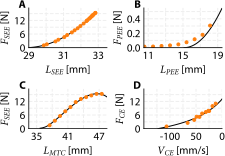
\includegraphics[keepaspectratio]{../figures/r_insitu_fit.pdf}}

}

\caption{\label{fig-r-insitu-fit}\textbf{Representative example of
experimental \emph{in situ} data of rat 1 for the SEE force-length
relationship (A), PEE force-length relationship (B), MTC force-length
relationship (C) and the CE force-velocity relationship (D).} The orange
dots depicts the experimental \emph{in situ} data and the solid black
line depicts the model fit.}

\end{figure}%

\begin{figure}[H]

\centering{

\pandocbounded{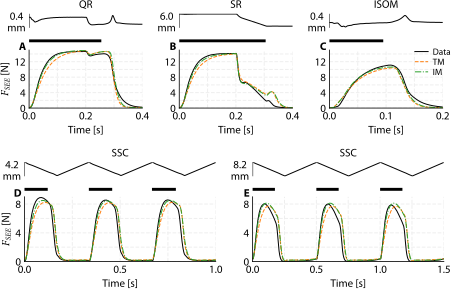
\includegraphics[keepaspectratio]{../figures/r_ssc_exp.pdf}}

}

\caption{\label{fig-r-ssc-exp}\textbf{Representative example of
experimental \emph{in situ} data and simulation results of rat 1 for SEE
force over time during a quick-release experiment (A), step-ramp
experiment (B), isometric experiment (C) and two stretch-shortening
cycles (D \& E).} The simulation results were obtained by re-simulating
the experimental protocol with the MTC length and CE stimulation from
the experimental data as input and by using either the parameter set
obtained with the traditional method (TM; orange dashed line) or the
improved method (IM; green dash-dotted line). For each panel, the top
plot represents MTC length over time, with the bar indicating its range
in mm. CE stimulation is maximal during the periods indicated by the
black bars and is `off' elsewhere.}

\end{figure}%

\section{Discussion}\label{discussion}

The aim of this study was to evaluate the accuracy of estimating
contraction and excitation dynamics parameter values on the basis of
data collected in commonly used experimental protocols. In real
experiments, the actual parameter values are unknown, making it
impossible to directly assess estimation accuracy. In this study, we
took a different approach: using a Hill-type MTC model with parameter
values obtained from literature we generated synthetic `data' by
simulating quick-release, step-ramp, and isometric experiments. We then
estimated all important contraction and excitation dynamics parameter
values by using the synthetic data. Since the actual parameter values
were known in this case, we could assess how accurately they were
retrieved. Two different estimation methods were compared. The first was
the traditional method, commonly used in the literature, which does not
account for muscle fibre shortening during quick-release experiments.
The second was an improved method that includes a correction for muscle
fibre shortening during the quick release. Both methods developed in
this study---designed to estimate contraction and excitation dynamics
parameters from quick-release, step-ramp, and isometric experiments
using servomotors---are made available as an open-source toolbox. In the
remainder of this paper, we will discuss 1) the difference between the
two methods; 2) the robustness of the improved method and 3) the
implications for muscle modelling.

In quick-release experiments using servomotors, muscle fibres shorten,
even within the short duration of the release. Obviously, the extent of
muscle fibre shortening depends on the duration of the quick-release.
Consequently, the longer the quick-release, the more important it
becomes to account for muscle fibre shortening when estimating SEE
stiffness (see \quartosuppfigref{suppfig-ksee-qr-duration}). For a
typical quick-release duration of 10 ms, we found that muscle fibre
shortening was nearly 25\% of MTC shortening (and thus 33\% of SEE
shortening), resulting in an underestimation of SEE stiffness by
approximately 35\%. This finding is important, especially in studies
aiming to estimate SEE energy storage from SEE force or length, since
energy storage estimates scale linearly with SEE stiffness. Although SEE
was substantially underestimated with the traditional method, this had
minimal effect on the estimated parameter values of the PEE and CE
force-length relationships and the CE force-velocity relationship, but
impacted the estimated excitation dynamics parameter values. The
improved method, in turn, yielded SEE stiffness values close to the
actual ones and substantially enhanced the estimates of the other
parameter values.

Our sensitivity analysis revealed substantial interdependencies between
certain parameters. Particularly, we observed high sensitivity of
estimated parameter values to variations in the maximal isometric CE
force (\(F_{CE}^{max}\)) and the SEE slack length (\(L_{SEE}^0\))
parameter values. Despite this sensitivity, it is important to note that
these parameters were accurately estimated even from perturbed
experimental data. This was true in general: contraction and excitation
dynamics parameter values were quite robust against shifts in the MTC
force-length relationship of the simulated data according to the Monte
Carlo simulations. These findings indicate the robustness of the
improved method.

We applied both the traditional and the improved method to \emph{in
situ} data from quick-release, step-ramp, and isometric experiments on
rat m. gastrocnemius medialis. The improved method yielded substantially
higher estimates of SEE stiffness compared to the traditional method
(67\% on average). Using parameter sets from both methods, we simulated
the quick-release, step-ramp, and isometric experiments, as well as
independent stretch-shortening cycles, all with experimentally obtained
MTC length and CE stimulation over time as input to the model. With
parameter estimates obtained with the traditional method, the root mean
squared difference between predicted and experimentally measured force
was about 5.6\% of maximal CE force, averaged across all rats and
experiments; with parameter estimates obtained with the improved method
this was only 3.9\%. The small difference between predicted and
experimentally observed force over time with parameters from the
improved method suggests that muscle force can be accurately predicted
with a Hill-type MTC model across a wide variety of contractions. This
is a remarkable finding for two reasons. First, the Hill-type MTC model
is obviously a simplification of real muscle, abstracting the muscle
belly, aponeurosis, and tendon into the CE, SEE, and PEE components, and
thus does not account for certain complexities (e.g., non-constant
pennation angle, muscle inhomogeneities, etc.). Second, the Hill-type
MTC model used in this study consists of 26 parameters, of which only 10
values were estimated. This means that all other parameters were left
suboptimal. Despite these simplifications, the model was able to
accurately predict muscle behaviour, demonstrating that a relatively
simple model with a limited number of estimated parameter values can
still capture important aspects of muscle dynamics.

In conclusion, our results demonstrate that the improved parameter
estimation method provides accurate and robust estimates of contraction
and excitation dynamics properties, offering a reliable approach for
muscle property estimation in both biomechanical and muscle physiology
research. The approach that we designed in this study is made available
as an open-source toolbox
(\url{https://github.com/edwinreuvers/mp-estimator}).

\newpage{}

\phantomsection

\section*{Acknowledgments}\label{acknowledgments}
\addcontentsline{toc}{section}{Acknowledgments}

The authors thank Maarten F. Bobbert for helpful comments on a draft of
the paper. The authors also thank Koen K. Lemaire for insightful
discussions.

\phantomsection

\section*{Funding}\label{funding}
\addcontentsline{toc}{section}{Funding}

This work was funded by The Dutch Research Council (NWO)~{[}21728 to
D.A.K.{]}.

\phantomsection

\section*{Data and resource
availability}\label{data-and-resource-availability}
\addcontentsline{toc}{section}{Data and resource availability}

All data, code, and materials used in this study are openly available:

\begin{itemize}
\item
  \textbf{GitHub repository:} All raw data, processed data, and analysis
  code are hosted on GitHub at
  \url{https://github.com/edwinreuvers/acc-mp-estimation}.
\item
  \textbf{Reproducible analysis website:} Full analysis pipeline ---
  including data, analysis code, and figure/table generation --- is
  available at
  \url{https://edwinreuvers.github.io/publications/acc-mp-estimation}.
\end{itemize}

\newpage{}

\newpage{}

\phantomsection

\section*{Glossary}\label{glossary}
\addcontentsline{toc}{section}{Glossary}

\begin{longtable}[]{@{}
  >{\raggedright\arraybackslash}p{(\linewidth - 2\tabcolsep) * \real{0.1111}}
  >{\raggedright\arraybackslash}p{(\linewidth - 2\tabcolsep) * \real{0.8889}}@{}}
\toprule\noalign{}
\begin{minipage}[b]{\linewidth}\raggedright
Symbol
\end{minipage} & \begin{minipage}[b]{\linewidth}\raggedright
Description
\end{minipage} \\
\midrule\noalign{}
\endhead
\bottomrule\noalign{}
\endlastfoot
\(a\) & Hill constant \\
\(b\) & Hill constant \\
\(b_{min}^{scale}\) & Minimal scale factor of \(b\) (i.e., the minimal
value of \(b_{scale}\)) \\
\(b_{shape}\) & Determines the steepness of the relation between
\(b_{scale}\) and \(q\) \\
\(F_{asymp}\) & Oblique asymptote of the eccentric part of the CE
force-velocity relationship \\
\(F_{CE}^{max}\) & Maximum isometric CE force \\
\(k_{PEE}\) & Scales the PEE stiffness \\
\(k_{SEE}\) & Scales the SEE stiffness \\
\(L_{CE}^{opt}\) & CE length at which CE can produce maximal isometric
force \\
\(L_{PEE}^0\) & PEE slack length \\
\(L_{SEE}^0\) & SEE slack length \\
\(r_{as}\) & Slope of the slanted asymptote of the eccentric part of the
CE force-velocity relationship \\
\(r_{slope}\) & Ratio between the eccentric and concentric derivatives
of \(\frac{dF_{CE}^{rel}}{dv_{CE}^{rel}}\) @ \(v_{CE}=0\) \\
\(w\) & Determines the width of the CE force-length relationship \\
\(a_{act}\) & Determines the steepness of the relation between
\(\gamma\) and \(q\) \\
\(b_{act,1}\) & Determines together with \(b_{act,1}\) and \(b_{act,3}\)
the \(pCa^{2+}\) level at which \(q=0.5\) \\
\(b_{act,2}\) & Determines together with \(b_{act,2}\) and \(b_{act,3}\)
the \(pCa^{2+}\) level at which \(q=0.5\) \\
\(b_{act,3}\) & Determines together with \(b_{act,1}\) and \(b_{act,2}\)
the \(pCa^{2+}\) level at which \(q=0.5\) \\
\(k_{Ca}\) & Relates \(\gamma\) to the actual \(Ca^{2+}\)
concentration \\
\(\gamma_0\) & Minimal value of \(\gamma\) \\
\(q_0\) & Minimal value \(q\) \\
\(\tau_{act}\) & Activation time constant of the calcium dynamics \\
\(\tau_{deact}\) & Deactivation time constant of the calcium dynamics \\
\end{longtable}

\newpage{}

\phantomsection

\section*{References}\label{references}
\addcontentsline{toc}{section}{References}

\phantomsection\label{refs}
\begin{CSLReferences}{1}{1}
\bibitem[\citeproctext]{ref-aubert_tension-length_1951}
\textbf{Aubert, X., Roquet, M. L. and Van der Elst, J.} (1951).
\href{https://doi.org/10.3109/13813455109145002}{The {Tension}-{Length}
{Diagram} of the {Frog}'s {Sartorius} {Muscle}}. \emph{Archives
Internationales de Physiologie} \textbf{59}, 239--241.

\bibitem[\citeproctext]{ref-blix_lange_1892}
\textbf{Blix, M.} (1892).
\href{https://doi.org/10.1111/j.1748-1716.1892.tb00660.x}{Die {Länge}
und die {Spannung} des {Muskels}}. \emph{Skandinavisches Archiv Für
Physiologie} \textbf{3}, 295--318.

\bibitem[\citeproctext]{ref-blix_lange_1893}
\textbf{Blix, M.} (1893).
\href{https://doi.org/10.1111/j.1748-1716.1893.tb00749.x}{Die {Länge}
und die {Spannung} des {Muskels}}. \emph{Skandinavisches Archiv Für
Physiologie} \textbf{4}, 399--409.

\bibitem[\citeproctext]{ref-blumel_determining_2012}
\textbf{Blümel, M., Hooper, S. L., Guschlbauerc, C., White, W. E. and
Büschges, A.} (2012).
\href{https://doi.org/10.1007/s00422-012-0531-5}{Determining all
parameters necessary to build {Hill}-type muscle models from experiments
on single muscles}. \emph{Biological Cybernetics} \textbf{106},
543--558.

\bibitem[\citeproctext]{ref-bobbert_force-length_1990}
\textbf{Bobbert, M. F., Ettema, G. C. and Huijing, P. A.} (1990).
\href{https://doi.org/10.1007/BF00357621}{The force-length relationship
of a muscle-tendon complex: Experimental results and model
calculations}. \emph{European Journal of Applied Physiology and
Occupational Physiology} \textbf{61}, 323--329.

\bibitem[\citeproctext]{ref-bortolotto_mhc_2000}
\textbf{Bortolotto, S. K., Cellini, M., Stephenson, D. G. and
Stephenson, G. M. M.} (2000).
\href{https://doi.org/10.1152/ajpcell.2000.279.5.C1564}{{MHC} isoform
composition and {Ca2}+- or {Sr2}+-activation properties of rat skeletal
muscle fibers}. \emph{American Journal of Physiology-Cell Physiology}
\textbf{279}, C1564--C1577.

\bibitem[\citeproctext]{ref-burkholder_sarcomere_2001}
\textbf{Burkholder, T. J. and Lieber, R. L.} (2001).
\href{https://doi.org/10.1242/jeb.204.9.1529}{Sarcomere {Length}
{Operating} {Range} of {Vertebrate} {Muscles} {During} {Movement}}.
\emph{Journal of Experimental Biology} \textbf{204}, 1529--1536.

\bibitem[\citeproctext]{ref-cecchi_force-velocity_1978}
\textbf{Cecchi, G., Colomo, F. and Lombardi, V.} (1978).
\href{https://doi.org/10.1113/jphysiol.1978.sp012570}{Force-velocity
relation in normal and nitrate-treated frog single muscle fibres during
rise of tension in an isometric tetanus.} \emph{The Journal of
Physiology} \textbf{285}, 257--273.

\bibitem[\citeproctext]{ref-ebashi_calcium_1968}
\textbf{Ebashi, S. and Endo, M.} (1968).
\href{https://doi.org/10.1016/0079-6107(68)90023-0}{Calcium and muscle
contraction}. \emph{Progress in Biophysics and Molecular Biology}
\textbf{18}, 123--183.

\bibitem[\citeproctext]{ref-gordon_variation_1966}
\textbf{Gordon, A. M., Huxley, A. F. and Julian, F. J.} (1966).
\href{https://doi.org/10.1113/jphysiol.1966.sp007909}{The variation in
isometric tension with sarcomere length in vertebrate muscle fibres}.
\emph{The Journal of Physiology} \textbf{184}, 170--192.

\bibitem[\citeproctext]{ref-hatze_myocybernetic_1981}
\textbf{Hatze, H.} (1981). \emph{Myocybernetic control models of
skeletal muscle}. Pretoria: University of South Africa.

\bibitem[\citeproctext]{ref-hill_length_1925}
\textbf{Hill, A. V.} (1925).
\href{https://doi.org/10.1113/jphysiol.1925.sp002242}{Length of muscle,
and the heat and tension developed in an isometric contraction}.
\emph{The Journal of Physiology} \textbf{60}, 237--263.

\bibitem[\citeproctext]{ref-hill_heat_1938}
\textbf{Hill, A. V.} (1938).
\href{https://doi.org/10.1098/rspb.1938.0050}{The heat of shortening and
the dynamic constants of muscle}. \emph{Proceedings of the Royal Society
of London. B. Biological Sciences} \textbf{126}, 136--195.

\bibitem[\citeproctext]{ref-hill_series_1950}
\textbf{Hill, A. V.} (1950).
\href{https://doi.org/10.1098/rspb.1950.0035}{The series elastic
componet of muscle}. \emph{Proceedings of the Royal Society of London.
B. Biological Sciences} \textbf{137}, 273--280.

\bibitem[\citeproctext]{ref-katz_relation_1939}
\textbf{Katz, B.} (1939).
\href{https://doi.org/10.1113/jphysiol.1939.sp003756}{The relation
between force and speed in muscular contraction}. \emph{The Journal of
Physiology} \textbf{96}, 45--64.

\bibitem[\citeproctext]{ref-kistemaker_length-dependent_2005}
\textbf{Kistemaker, D. A., Van Soest, A. (Knoek). J. and Bobbert, M. F.}
(2005).
\href{https://doi.org/10.1016/j.jbiomech.2004.08.025}{Length-dependent
{[}{Ca2}+{]} sensitivity adds stiffness to muscle}. \emph{Journal of
Biomechanics} \textbf{38}, 1816--1821.

\bibitem[\citeproctext]{ref-kistemaker_limiting_2023}
\textbf{Kistemaker, D. A., Terwiel, R. M., Reuvers, E. D. H. M. and
Bobbert, M. F.} (2023).
\href{https://doi.org/10.1152/japplphysiol.00733.2021}{Limiting radial
pedal forces greatly reduces maximal power output and efficiency in
sprint cycling; an optimal control study}. \emph{Journal of Applied
Physiology} \textbf{134}, 980--991.

\bibitem[\citeproctext]{ref-lemaire_comparison_2016}
\textbf{Lemaire, K. K., Baan, G. C., Jaspers, R. T. and Soest, A. J.
`Knoek'. van} (2016).
\href{https://doi.org/10.1242/jeb.144394}{Comparison of the validity of
{Hill} and {Huxley} muscle--tendon complex models using experimental
data obtained from rat m. Soleus~in situ}. \emph{Journal of Experimental
Biology} \textbf{219}, 2228--2228.

\bibitem[\citeproctext]{ref-levin_viscous_1927}
\textbf{Levin, A. and Wyman, J.} (1927).
\href{https://doi.org/10.1098/rspb.1927.0014}{The viscous elastic
properties of muscle}. \emph{Proceedings of the Royal Society of London.
Series B, Containing Papers of a Biological Character} \textbf{101},
218--243.

\bibitem[\citeproctext]{ref-petrofsky_influence_1981}
\textbf{Petrofsky, J. S. and Phillips, C. A.} (1981).
\href{https://doi.org/10.1016/0021-9290(81)90039-7}{The influence of
temperature, initial length and electrical activity on the
force-velocity relationship of the medial gastrocnemius muscle of the
cat}. \emph{Journal of Biomechanics} \textbf{14}, 297--306.

\bibitem[\citeproctext]{ref-rack_effects_1969}
\textbf{Rack, P. M. H. and Westbury, D. R.} (1969).
\href{https://doi.org/10.1113/jphysiol.1969.sp008923}{The effects of
length and stimulus rate on tension in the isometric cat soleus muscle}.
\emph{The Journal of Physiology} \textbf{204}, 443--460.

\bibitem[\citeproctext]{ref-reuvers_maximising_2025}
\textbf{Reuvers, E. D. H. M., Maas, H., Noort, W., Bobbert, M. F. and
Kistemaker, D. A.} (2025).
\href{https://doi.org/10.1101/2025.09.25.678481}{Maximising average
mechanical power output during stretch-shortening cycles of rat medial
gastrocnemius muscle}.

\bibitem[\citeproctext]{ref-rijkelijkhuizen_forcevelocity_2003}
\textbf{Rijkelijkhuizen, J. M., Ruiter, C. J. de, Huijing, P. A. and
Haan, A. de} (2003).
\href{https://doi.org/10.1007/s00424-003-1052-9}{Force/velocity curves
of fast oxidative and fast glycolytic parts of rat medial gastrocnemius
muscle vary for concentric but not eccentric activity}. \emph{Pflügers
Archiv} \textbf{446}, 497--503.

\bibitem[\citeproctext]{ref-van_soest_contribution_1993}
\textbf{Soest, A. J. van and Bobbert, M. F.} (1993).
\href{https://doi.org/10.1007/BF00198959}{The contribution of muscle
properties in the control of explosive movements}. \emph{Biological
Cybernetics} \textbf{69}, 195--204.

\bibitem[\citeproctext]{ref-stephenson_effects_1982}
\textbf{Stephenson, D. G. and Williams, D. A.} (1982).
\href{https://doi.org/10.1113/jphysiol.1982.sp014473}{Effects of
sarcomere length on the force---{pCa} relation in fast- and slow-twitch
skinned muscle fibres from the rat}. \emph{The Journal of Physiology}
\textbf{333}, 637--653.

\bibitem[\citeproctext]{ref-stern_computer_1974}
\textbf{Stern, J. T.} (1974).
\href{https://doi.org/10.1016/0021-9290(74)90004-9}{Computer modelling
of gross muscle dynamics}. \emph{Journal of Biomechanics} \textbf{7},
411--428.

\bibitem[\citeproctext]{ref-van_soest_consequences_2005}
\textbf{Van Soest, A. J., Gföhler, M. and Casius, L. J. R.} (2005).
\href{https://journals.lww.com/acsm-msse/fulltext/2005/05000/consequences_of_ankle_joint_fixation_on_fes.14.aspx}{Consequences
of {Ankle} {Joint} {Fixation} on {FES} {Cycling} {Power} {Output}: {A}
{Simulation} {Study}}. \emph{Medicine \& Science in Sports \& Exercise}
\textbf{37},.

\bibitem[\citeproctext]{ref-walker_i_1974}
\textbf{Walker, S. M. and Schrodt, G. R.} (1974).
\href{https://doi.org/10.1002/ar.1091780107}{I segment lengths and thin
filament periods in skeletal muscle fibers of the rhesus monkey and the
human}. \emph{The Anatomical Record} \textbf{178}, 63--81.

\bibitem[\citeproctext]{ref-woittiez_three-dimensional_1984}
\textbf{Woittiez, R. D., Huijing, P. A., Boom, H. B. K. and Rozendal, R.
H.} (1984). \href{https://doi.org/10.1002/jmor.1051820107}{A
three-dimensional muscle model: {A} quantified relation between form and
function of skeletal muscles}. \emph{Journal of Morphology}
\textbf{182}, 95--113.

\bibitem[\citeproctext]{ref-zajac_muscle_1989}
\textbf{Zajac, F. E.} (1989). Muscle and tendon: Properties, models,
scaling, and application to biomechanics and motor control.
\emph{Critical reviews in biomedical engineering} \textbf{17}, 359--411.

\bibitem[\citeproctext]{ref-van_zandwijk_evaluation_1997}
\textbf{Zandwijk, J. P. van, Baan, G. C., Bobbert, M. F. and Huijing, P.
A.} (1997). \href{https://doi.org/10.1007/s004220050388}{Evaluation of a
self-consistent method for calculating muscle parameters from a set of
isokinetic releases}. \emph{Biological Cybernetics} \textbf{77},
277--281.

\end{CSLReferences}

\appendix
\phantomsection

\section*{Supplementary material}\label{supplementary-material}
\addcontentsline{toc}{section}{Supplementary material}

\setcounter{subsection}{0} % Reset subsection counter

% Define subsection numbering in appendix as S1, S2, ...
\renewcommand{\thesubsection}{S\arabic{subsection}}

\renewcommand{\thetable}{S\arabic{table}}
\setcounter{table}{0}

\subsection{Supplemental figures}\label{supplemental-figures}

\begin{suppfig}[H]

\centering{

\pandocbounded{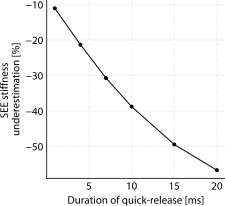
\includegraphics[keepaspectratio]{../figures/s_servo_vs_lever.pdf}}

}

\caption{\label{suppfig-servo-vs-lever}\textbf{Comparison between a
length-controlled step-ramp experiment and a force-controlled
quick-release experiment.} In length-controlled step-ramp experiment
(left), MTC length over time is imposed using a servomotor, while SEE
force is measured. MTC velocity is computed at the time instance at
which SEE force is near constant. In the force-controlled quick-release
experiment (right), SEE force over time is imposed via a lever, while
MTC length is measured. MTC velocity is computed at the time instance
where MTC velocity is maximal after the change in SEE force. Both
methods yield one datapoint (depicted with the orange dot) of the
force-velocity relationship.}

\end{suppfig}%

\begin{suppfig}[H]

\centering{

\pandocbounded{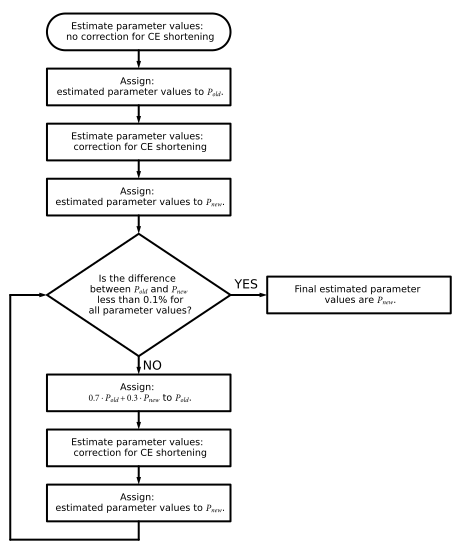
\includegraphics[keepaspectratio]{../figures/s_flowchart.pdf}}

}

\caption{\label{suppfig-flowchart}\textbf{Flowchart of the improved
method.} Using the improved method, parameter values were estimated
until the change in all parameter values was less than 0.1\%.}

\end{suppfig}%

\begin{suppfig}[H]

\centering{

\pandocbounded{\includegraphics[keepaspectratio]{../figures/s_ksee_qr_duration.pdf}}

}

\caption{\label{suppfig-ksee-qr-duration}\textbf{Relationship between
quick-release duration and SEE stiffness understimation}. When the
duration of the quick-release increases, the underestimation of SEE
stiffness increases.}

\end{suppfig}%

\newpage{}

\subsection{Supplemental tables}\label{supplemental-tables}

\begin{supptbl}

\caption{\label{supptbl-overview}MTC parameter values obtained from
literature to simulate data.}

\centering{

\begin{tabular}{|l|l|c|c|c|l|} \hline
 \bfseries Parameter & \bfseries Unit & \bfseries GM1 & \bfseries GM2 & \bfseries GM3 & \bfseries Reference \\ \hline
\multicolumn{6}{|l|}{\itshape Contraction dynamics} \\ \hline
$a$ & N & 2.68 & 1.80 & 2.58 & <span class="citation" data-cites="van\_zandwijk\_evaluation\_1997">van Zandwijk et al. (<a href="\#ref-van\_zandwijk\_evaluation\_1997" role="doc-biblioref" aria-expanded="false">1997</a>)</span> \\ \hline
$b$ & mm & 41.6 & 24.8 & 41.8 & <span class="citation" data-cites="van\_zandwijk\_evaluation\_1997">van Zandwijk et al. (<a href="\#ref-van\_zandwijk\_evaluation\_1997" role="doc-biblioref" aria-expanded="false">1997</a>)</span> \\ \hline
$b_{scale}^{min}$  & -  &\multicolumn{3}{c|}{0.100} & <span class="citation" data-cites="van\_soest\_contribution\_1993">van Soest and Bobbert (<a href="\#ref-van\_soest\_contribution\_1993" role="doc-biblioref" aria-expanded="false">1993</a>)</span> \\ \hline 
$b_{shape}$  & -  &\multicolumn{3}{c|}{22.0} & <span class="citation" data-cites="van\_soest\_contribution\_1993">van Soest and Bobbert (<a href="\#ref-van\_soest\_contribution\_1993" role="doc-biblioref" aria-expanded="false">1993</a>)</span> \\ \hline 
$F_{asymp}$  & -  &\multicolumn{3}{c|}{1.50} & <span class="citation" data-cites="rijkelijkhuizen\_forcevelocity\_2003">Rijkelhuizen et al. (<a href="\#ref-rijkelijkhuizen\_forcevelocity\_2003" role="doc-biblioref" aria-expanded="false">2003</a>)</span> \\ \hline 
$F_{CE}^{max}$ & N & 13.4 & 13.8 & 12.3 & <span class="citation" data-cites="van\_zandwijk\_evaluation\_1997">van Zandwijk et al. (<a href="\#ref-van\_zandwijk\_evaluation\_1997" role="doc-biblioref" aria-expanded="false">1997</a>)</span> \\ \hline
$k_{PEE}$  & N/mm\textsuperscript{2}  & 213  & 165  & 511  & <span class="citation" data-cites="van\_zandwijk\_evaluation\_1997">van Zandwijk et al. (<a href="\#ref-van\_zandwijk\_evaluation\_1997" role="doc-biblioref" aria-expanded="false">1997</a>)</span> \\ \hline 
$k_{SEE}$  & N/mm\textsuperscript{2}  & 4220  & 3640  & 3470  & <span class="citation" data-cites="van\_zandwijk\_evaluation\_1997">van Zandwijk et al. (<a href="\#ref-van\_zandwijk\_evaluation\_1997" role="doc-biblioref" aria-expanded="false">1997</a>)</span> \\ \hline 
$L_{CE}^{opt}$ & mm & 13.2 & 12.3 & 11.2 & <span class="citation" data-cites="van\_zandwijk\_evaluation\_1997">van Zandwijk et al. (<a href="\#ref-van\_zandwijk\_evaluation\_1997" role="doc-biblioref" aria-expanded="false">1997</a>)</span> \\ \hline
$L_{PEE}^0$ & mm & 13.9 & 13.2 & 13.4 & <span class="citation" data-cites="van\_zandwijk\_evaluation\_1997">van Zandwijk et al. (<a href="\#ref-van\_zandwijk\_evaluation\_1997" role="doc-biblioref" aria-expanded="false">1997</a>)</span> \\ \hline
$L_{SEE}^0$ & mm & 28.3 & 30.3 & 26.5 & <span class="citation" data-cites="van\_zandwijk\_evaluation\_1997">van Zandwijk et al. (<a href="\#ref-van\_zandwijk\_evaluation\_1997" role="doc-biblioref" aria-expanded="false">1997</a>)</span> \\ \hline
$r_{as}$    & -    & $3.71 \cdot 10^{-3}$    & $5.45 \cdot 10^{-3}$   & $3.16 \cdot 10^{-3}$  & Arbitrary small value \\ \hline 
\multicolumn{6}{|l|}{\itshape Excitation dynamics} \\ \hline
$r_{slope}$  & mm  &\multicolumn{3}{c|}{2.00} & <span class="citation" data-cites="katz\_relation\_1939">Katz (1939) (<a href="\#ref-katz\_relation\_1939" role="doc-biblioref" aria-expanded="false">1939</a>)</span> \\ \hline 
$w$  & -  &\multicolumn{3}{c|}{0.50} & <span class="citation" data-cites="burkholder\_sarcomere\_2001">Burkholder and Lieber (<a href="\#ref-burkholder\_sarcomere\_2001" role="doc-biblioref" aria-expanded="false">2001</a>)</span> \\ \hline 
$a_{act}$  & ?  &\multicolumn{3}{c|}{-7.37} & <span class="citation" data-cites="bortolotto\_mhc\_2000">Bortolotto et al. (<a href="\#ref-bortolotto\_mhc\_2000" role="doc-biblioref" aria-expanded="false">2000</a>)</span> \\ \hline 
$b_{act,1}$  & ?  &\multicolumn{3}{c|}{5.17} & <span class="citation" data-cites="bortolotto\_mhc\_2000">Bortolotto et al. (<a href="\#ref-bortolotto\_mhc\_2000" role="doc-biblioref" aria-expanded="false">2000</a>)</span> \\ \hline 
$b_{act,2}$  & ?  &\multicolumn{3}{c|}{0.596} & <span class="citation" data-cites="stephenson\_effects\_1982">Stephenson and Williams (<a href="\#ref-stephenson\_effects\_1982" role="doc-biblioref" aria-expanded="false">1982</a>)</span> \\ \hline 
$b_{act,3}$  & ?  &\multicolumn{3}{c|}{0.00} & <span class="citation" data-cites="stephenson\_effects\_1982">Stephenson and Williams (<a href="\#ref-stephenson\_effects\_1982" role="doc-biblioref" aria-expanded="false">1982</a>)</span> \\ \hline 
$kCa$  & mol/L  &\multicolumn{3}{c|}{$8.00 \cdot 10^{-6}$} & <span class="citation" data-cites="kistemaker\_length-dependent\_2005">Kistemaker et al. (<a href="\#ref-kistemaker\_length-dependent\_2005" role="doc-biblioref" aria-expanded="false">2005</a>)</span> \\ \hline 
$\gamma_0$  & -  &\multicolumn{3}{c|}{$1.00 \cdot 10^{-5}$} & Arbitrary small value \\ \hline 
$q_0$  & -  &\multicolumn{3}{c|}{$5.00 \cdot 10^{-3}$} & <span class="citation" data-cites="hatze\_myocybernetic\_1981">Hatze (<a href="\#ref-hatze\_myocybernetic\_1981" role="doc-biblioref" aria-expanded="false">1981</a>)</span> \\ \hline 
$\tau_{act}$  & ms  &\multicolumn{3}{c|}{27.0} & <span class="citation" data-cites="van\_zandwijk\_evaluation\_1997">van Zandwijk et al. (<a href="\#ref-van\_zandwijk\_evaluation\_1997" role="doc-biblioref" aria-expanded="false">1997</a>)</span> \\ \hline 
$\tau_{deact}$  & ms  &\multicolumn{3}{c|}{27.0} & <span class="citation" data-cites="van\_zandwijk\_evaluation\_1997">van Zandwijk et al. (<a href="\#ref-van\_zandwijk\_evaluation\_1997" role="doc-biblioref" aria-expanded="false">1997</a>)</span> \\ \hline 
\end{tabular}

}

\end{supptbl}%

\begin{supptbl}

\caption{\label{supptbl-insitu}Estimated parameter values of the
experimentally measured in situ data using both the traditional as well
as the improved method.}

\centering{

\begin{tabular}{|l|c|c|c|c|c|c|c|} \hline
  & & \multicolumn{3}{c|}{\itshape Traditional method} & \multicolumn{3}{c|}{\itshape Improved method} \\ \hline
  \bfseries Parameter & \bfseries Unit & \bfseries Rat 1 & \bfseries Rat 2 & \bfseries Rat 3 & \bfseries Rat 1 & \bfseries Rat 2 & \bfseries Rat 3 \\ \hline
$a$ & N & 8.90 & 11.3 & 10.5 & 8.82 & 10.0 & 11.0 \\ \hline
$b$ & mm & 76.7 & 108 & 84.6 & 81.9 & 105 & 90.6 \\ \hline
$F_{CE}^{max}$ & N & 15.6 & 14.1 & 17.1 & 15.5 & 14.1 & 17.0 \\ \hline
$k_{PEE}$ & N/mm<sup>2</sup> & 9.83 & 7.25 & 21.9 & 28.7 & 24.1 & 34.8 \\ \hline
$k_{SEE}$ & N/mm<sup>2</sup> & 608 & 688 & 654 & 952 & 1260 & 1050 \\ \hline
$L_{CE}^{opt}$ & mm & 12.4 & 12.9 & 12.3 & 13.7 & 14.7 & 13.3 \\ \hline
$L_{PEE}^0$ & mm & 12.4 & 12.4 & 13.3 & 15.1 & 15.6 & 14.5 \\ \hline
$L_{SEE}^0$ & mm & 29.0 & 29.7 & 25.1 & 28.8 & 29.3 & 25.2 \\ \hline
$\tau_{act}$ & ms & 43.0 & 32.4 & 23.6 & 55.2 & 57.7 & 41.6 \\ \hline
$\tau_{deact}$ & ms & 23.8 & 20.9 & 19.7 & 27.1 & 25.3 & 22.4 \\ \hline
\end{tabular}

}

\end{supptbl}%

\begin{supptbl}

\caption{\label{supptbl-rmsd}Root mean squared differences between
experimentally measured SEE force histories and those predicted by
Hill-type MTC model after estimating all contraction and excitation
dynamics parameter values.}

\centering{

\begin{tabular}{|l|c|c|c|c|c|c|c|c|} \hline
 & \multicolumn{4}{c|}{\itshape Traditional method} & \multicolumn{4}{c|}{\itshape Improved method} \\ \hline
 & \bfseries QR & \bfseries SR & \bfseries ISOM & \bfseries SSC & \bfseries QR & \bfseries SR & \bfseries ISOM & \bfseries SSC \\ \hline
Rat 1 & 5.6 ± 3.4 & 5.6 ± 0.8 & 6.8 ± 3.2 & 6.2 ± 3.0 & 3.3 ± 1.5 & 2.8 ± 0.9 & 5.4 ± 3.0 & 5.4 ± 3.1 \\ \hline
Rat 2 & 4.2 ± 1.5 & 5.0 ± 0.6 & 4.3 ± 1.6 & 4.6 ± 2.2 & 2.7 ± 1.6 & 2.1 ± 0.5 & 4.2 ± 2.6 & 4.2 ± 2.0 \\ \hline
Rat 3 & 6.4 ± 2.3 & 6.8 ± 1.0 & 6.1 ± 2.1 & 5.5 ± 2.7 & 4.2 ± 1.8 & 2.6 ± 0.5 & 4.9 ± 2.3 & 5.0 ± 2.7 \\ \hline
Avg ± Std & 5.4 ± 2.6 & 5.8 ± 1.1 & 5.7 ± 2.7 & 5.4 ± 2.7 & 3.4 ± 1.8 & 2.5 ± 0.7 & 4.8 ± 2.7 & 4.9 ± 2.7 \\ \hline
\end{tabular}\break\hfill\footnotesize{Root mean squared differences are expressed as a percentage of the maximal isometric CE force ($F_{CE}^{max}$). Root mean squared differences were computed over the interval in which CE stimulation was maximal for the quick-release and step-ramp experiments and was computed over the interval from CE stimulation onset to 0.1 s after CE stimulation offset for the isometric experiments and the stretch-shortening cycles.}

}

\end{supptbl}%




\end{document}
